\documentclass[10pt,a4paper]{scrreprt}

%----------------------------------------------------------------------------------------
%	REQUIRED PACKAGES AND MISC CONFIGURATIONS
%----------------------------------------------------------------------------------------

\usepackage{graphicx} % Required for including images

\setcounter{secnumdepth}{-2} % Remove all section numbering

\usepackage{hyperref}
\usepackage{multicol} % Allows table cells to span multiple columns
\usepackage{longtable} % Allows the creation of tables that automatically wrap to the next page

\pagestyle{plain} % Use the plain page style for all headers and footers (only a page number)

\usepackage{scrhack} % Fixes compatibility issues between KOMA-Script and other packages

\usepackage{lastpage} % Required to determine the total number of pages

\usepackage{pdfpages}

%----------------------------------------------------------------------------------------
%	MARGINS
%----------------------------------------------------------------------------------------

\usepackage[
	top=2.5cm, % Top margin
	bottom=2.5cm, % Bottom margin
	inner=1.5cm, % Inner margin
	outer=3cm, % Outer margin
	footskip=1.4cm, % Space from the bottom margin to the baseline of the footer
	headsep=0.8cm, % Space from the top margin to the baseline of the header
	headheight=0.5cm, % Height of the header
	%showframe % Uncomment to show the frames around the margins for debugging purposes
]{geometry}


%----------------------------------------------------------------------------------------
%	FONTS & TYPOGRAPHY
%----------------------------------------------------------------------------------------

\usepackage[utf8]{inputenc} % Required for inputting international characters
\usepackage[T1]{fontenc} % Output font encoding for international characters

\usepackage[sfdefault, lf]{carlito} % Use the Carlito family of sans-serif fonts with lining figures

\DeclareUnicodeCharacter{200B}{ }

%----------------------------------------------------------------------------------------
%	COLOURS
%----------------------------------------------------------------------------------------

\usepackage{xcolor} % Required for defining and using custom colours

\definecolor{myorange}{RGB}{255, 117, 40}
\definecolor{mywhite}{RGB}{235, 238, 231}

\definecolor{mpigreen}{RGB}{17, 102, 86}
\definecolor{mpigrey}{RGB}{221, 222, 214}

% from https://cran.r-project.org/web/packages/unikn/vignettes/color_inst.html
\newcommand{\primarycolor}{mpigreen}
\newcommand{\secondarycolor}{mywhite}

% Table colours
\newcommand{\tbg}{gray} % Event background
\newcommand{\tfg}{white} % Event foreground (text)
\newcommand{\tbc}{gray!25} % Break background

% Talk types colours
\newcommand{\IScolor}{mpigreen!65} % Invited speaker
\newcommand{\CTcolor}{white} % Contributed talk
\newcommand{\KLcolor}{myorange!45} % Keynote lecture
\newcommand{\ITcolor}{yellow!25} % Invited talk

%----------------------------------------------------------------------------------------
%	LINKS
%----------------------------------------------------------------------------------------

\usepackage{hyperref} % Required for links

\hypersetup{
	colorlinks=false,
	%urlcolor=\primarycolor, % Colour for \url and \href links
	%linkcolor=\primarycolor, % Colour for \nameref links
	hidelinks, % Hide the default boxes around links
}

%----------------------------------------------------------------------------------------
%	TABLE DEFINITIONS
%----------------------------------------------------------------------------------------

\usepackage{array} % Required for manipulating table columns

\newcommand{\tablebreak}[2]{\rowcolor{\tbc} #1 & \multicolumn{4}{c|}{\bfseries #2} \\ \hline } % Timetable conference break row
\newcommand{\eventtype}[2]{#1 & \multicolumn{4}{c|}{\cellcolor{\tbg}\color{\tfg}\bfseries #2} \\ \hline } % Timetable conference event row

\newcolumntype{L}[1]{>{\raggedright\let\newline\\\arraybackslash\hspace{0pt}}m{#1}} % Define a new left-aligned (no justification) column type
\newcolumntype{C}[1]{>{\centering\let\newline\\\arraybackslash\hspace{0pt}}m{#1}} % Define a new centred column type
\newcolumntype{R}[1]{>{\raggedleft\let\newline\\\arraybackslash\hspace{0pt}}m{#1}} % Define a new right-aligned column type

\newcommand{\IS}[4]{#1 & \cellcolor{\IScolor}IS & {\bfseries#2}\newline #3 & & #4 \\ \hline} % Invited speaker row
\newcommand{\CT}[4]{#1 & \cellcolor{\CTcolor}CT & {\bfseries#2}\newline #3 & & #4 \\ \hline} % Contributed talk row
\newcommand{\KL}[4]{#1 & \cellcolor{\KLcolor}KL & {\bfseries#2}\newline #3 & & #4 \\ \hline} % Keynote lecture row
\newcommand{\IT}[4]{#1 & \cellcolor{\ITcolor}IT & {\bfseries#2}\newline #3 & & #4 \\ \hline} % Invited talk row
\newcommand{\tutorial}[4]{#1 & & {\bfseries#2}\newline #3 & & #4 \\ \hline} % Tutorial row

%----------------------------------------------------------------------------------------
%	CHAPTER STYLING
%----------------------------------------------------------------------------------------

\newdimen\mybarpadding
\mybarpadding=1.5em\relax % Horizontal padding between the coloured bar and chapter name

\RedeclareSectionCommand[% Adjust the spacing around the \chapter command
	afterskip=4em plus 1pt minus 1pt,% Vertical whitespace under chapters
	beforeskip=-1pt, % Vertical whitespace before chapters
	level=0,% Chapters are the top level command
	toclevel=0,% Chapters are the top level command
]{chapter}

\setkomafont{chapter}{\normalfont\normalsize\bfseries\Huge} % Chapter font style

\RedeclareSectionCommand[% Adjust the spacing around the \section command
	afterskip=6pt,% Vertical whitespace under sections
	beforeskip=3pt, % Vertical whitespace before chapters
	level=1,% Sections are the second level command
	toclevel=1,% Sections are the second level command
]{section}

%------------------------------------------------

\renewcommand{\chapterlinesformat}[3]{%
	\ifthispageodd{% Odd pages have the coloured bar to the left of the chapter title
		\hfill% Coloured bar fills available width
		\raisebox{-0.2em}{\makebox[0pt][r]{\textcolor{\primarycolor}{\rule{\paperwidth}{1em}}}}% Coloured bar
		\hspace{\mybarpadding}% Padding between the chapter title and colour bar
		\mbox{#3}% Chapter title
	}{% Even pages have the coloured bar to the right of the chapter title
		\mbox{#3}% Chapter title
		\hspace{\mybarpadding}% Padding between the chapter title and colour bar
		\raisebox{-0.2em}{\makebox[0pt][l]{\textcolor{\primarycolor}{\rule{\paperwidth}{1em}}}}% Coloured bar
	}%
}

%----------------------------------------------------------------------------------------
%	ABSTRACT STYLING
%----------------------------------------------------------------------------------------

\newcommand{\dosabstract}[4]{
\filbreak % Avoid page breaks within abstracts

\noindent
{\large \bfseries #1} % Title

\noindent
{\bfseries \itshape #2} % Author(s)	

\noindent
\textcolor{mpigrey}{#3} % Affiliation(s)

\vskip 0.2 cm
\noindent
#4 % Abstract text
\vskip 0.5 cm
}


% =======================================================================================
% =======================================================================================
% =======================================================================================


\begin{document}

\title{Day of Science}
\date{December 15, 2023}


%----------------------------------------------------------------------------------------
%	 COVER PAGE
%----------------------------------------------------------------------------------------

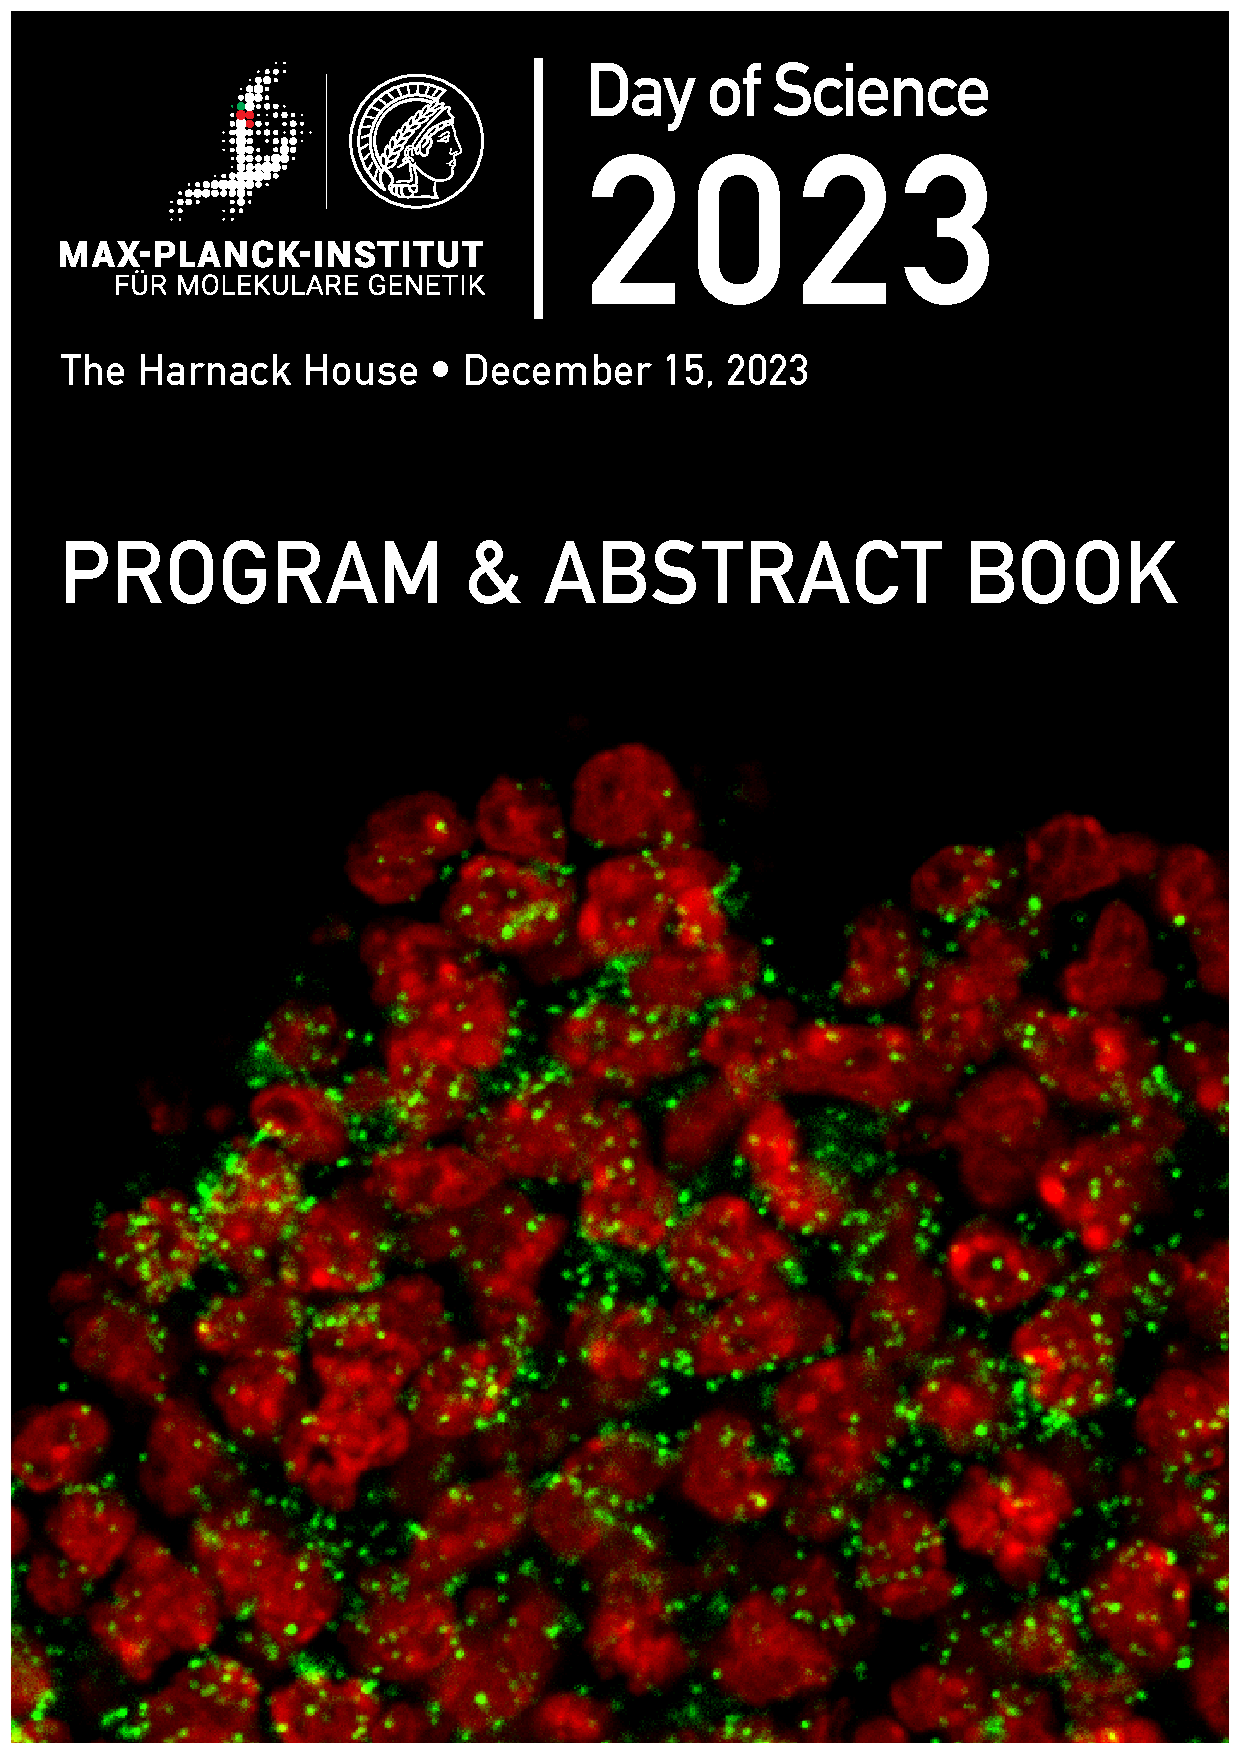
\includepdf{images/adri-cells.pdf}

%----------------------------------------------------------------------------------------
%	 TABLE OF CONTENTS
%----------------------------------------------------------------------------------------

\tableofcontents

%----------------------------------------------------------------------------------------
%	 ABOUT CONFERENCE
%----------------------------------------------------------------------------------------

\chapter{About}

\vskip 1 cm

\section*{Day of Science}

The annual Day of Science (DoS) aims to ...

\vskip 1 cm

\section*{Max Planck Institute for Molecular Genetics}

The DoS is organized by the ... of the Max Planck Institute for Molecular Genetics (MPIMG) ...

\vskip 1 cm

\section*{Organizing committee}

\begin{center}
	\begin{tabular}{l l l}
		Adriano Bolondi &  Anna A. Monaco &  Alessa Ringel\\
		Jakob Schweizer  &  Thomas R. Silvers &
	\end{tabular}
\end{center}

\vskip 1 cm

\section*{Special thanks}
	\begin{tabular}{l l l}
		Max Planck & Harnack-Haus & Minerva
	\end{tabular}

\vskip 2 cm

\noindent
{\small This conference booklet was generated using \LaTeX{}, adapted from a template created by Maxime Lucas. All information about the use and distribution of this template, and all related codes, can be found at \url{https://github.com/maximelucas/AMCOS_booklet}. The entire source code for the adapted template and its generation can be found at \url{https://github.com/t-silvers/dos_abstract_book}.}

%----------------------------------------------------------------------------------------
%	 SCHEDULE
%----------------------------------------------------------------------------------------

\chapter{Schedule}

%----------------------------------------------------------------------------------------
%	 LIST OF TALK ABSTRACTS
%----------------------------------------------------------------------------------------

% Abstract template
%\abstract
%	{} % Title
%	{} % Author(s)
%	{} % Tag, can be: empty, \KLtag (keynote lecture), \IStag (invited speaker), \CTtag (contributed talk) or \ITtag (invited talk)
%	{} % Affiliation(s)
%	{} % Abstract text

\chapter{List of Abstracts -- Talks}

\dosabstract{The causes and consequences of 3D-architectural changes at the onset of X-chromosome inactivation}{Alexandra Martitz, Edda Schulz}{<Lab missing>, Dpt. <Dpt missing>}{In the intricate realm of mammalian gene regulation, cis-regulatory elements play a crucial role in orchestrating precise gene expression during development. To exert their regulatory effect, they must come into physical contact with the promoters of their target genes, which is thought to be facilitated by loop extrusion. Here, ring-shaped cohesin complexes facilitate the contacts within defined regions of the genome, which are called topologically associating domains (TADs). To explore the intricate relationship between the cis-regulatory landscape, TAD structure, and gene expression, we employ the X inactivation centre (Xic) in mouse embryonic stem cells as a model system. The Xic regulates X-chromosome inactivation (XCI) in female mammals, in which one of the two X chromosomes is randomly chosen and silenced in early embryonic development to compensate for the double dosage of X-linked genes. Previous research has shown that the bipartite TAD structures at the Xic undergoes rewiring throughout development, exhibiting distinct patterns on the active and silenced X chromosomes. By using state-of-the-art techniques (i.e. Tiled-C, Tiled-MCC) to map the chromatin architecture at up to base-pair resolution, we have revealed nano-scale structures with unprecedent detail. Together with novel ChIPmentation data, we are able to show increased cohesin binding at activated sites as well as enhanced CTCF binding at rewired anchor sites. Together, our findings provide insights into the mechanisms of loop extrusion in regulating fine-scale chromatin architecture. }
\dosabstract{Genome-wide demographic analyses of balaenid whales revealed complex history of gene flow associated with past climate oscillation.}{Bai-Wei Lo, Francisca Martinez-Real, Stefan Mundlos}{<Lab missing>, Dpt. <Dpt missing>}{The balaenid whale, consisting of three species of right whales and the bowhead whale, represents an ancient and highly endangered lineage of marine mammals. In order to elucidate the evolutionary history of balaenid whales with respect to gene flow, a comprehensive analysis based on whole-genome data was conducted for all species within this group. Employing population genomic methodologies, we revealed the polytomic nature of extant right whales, identified passage of historical trans-equatorial migration, and provided estimates to the age of the group. Furthermore, we investigated the impact of glacial cycles on the connectivity of bowhead whale populations. Through the utilization of multiple complementary approaches to detect gene flow, we identified and characterized gene flow events from bowhead whales to North Atlantic right whales, offering detailed insights into the process. Lastly, we assessed the phenotypic consequences of interspecies gene flow. The outcomes of our study shed light on the intricate evolutionary history of modern balaenid whales, which have been profoundly shaped by ancient climate events.}
\dosabstract{Joint clustering and visualization of cells and genes for single-cell transcriptomics}{Clemens Kohl, Yan Zhao, Martin Vingron}{<Lab missing>, Dpt. <Dpt missing>}{Single-cell RNA-sequencing (scRNA-seq) allows researchers to study the heterogeneity of biological samples. Current methods however mainly focus on clustering the cells and attempt to determine the genes that define the clusters post-hoc through differential gene expression analysis and similar methods. This approach however often results in misleadingly low p-values and can find differences even in completely random data. Biclustering promises to solve this problem by simultaneously finding cell clusters and their respective marker genes. However, existing biclustering algorithms struggle with the higher noise and large size of scRNA-seq data and lack tools for a practical and concise visualization of results.  We here present two approaches on how Correspondence Analysis (CA) can be used to co-cluster cells and their respective marker genes in a single step, thereby solving the problems of current methods.  In order to tackle the task of identifying and annotating cell types in scRNA-seq data we developed Correspondence analysis based biclustering on Networks (CAbiNet). We build a graph connecting cells and genes in the noise and dimension reduced CA space by utilizing the Association Ratio to quantify the extent of how much the observed gene expression deviates from the expected expression in a cell. Clustering on this graph not only yields cell clusters and their cell type specific genes, but additionally allows us to visualize the cells and their defining marker genes in a single 2D plot that enables quick annotation and exploration of the obtained clusters. An additional advantage of this approach is that the graph could be extended to include additional data modalities such as scATAC-seq data.   Given the increasing size of scRNA-seq data, fast and highly scalable methods are required for analysis. We can furthermore exploit the highly directional geometry induced by CA to simultaneously cluster cells and their marker genes based on a total least squares regression approach that enables the analysis of even the largest datasets. }
\dosabstract{RiboSTS: a technology for combined single-cell sequencing of rRNA and mRNA}{Dmitrii Zagrebin, Matthew Kraushar}{<Lab missing>, Dpt. <Dpt missing>}{The ribosome is a multi-megadalton RNA-protein complex responsible for the translation of mRNAs into functional proteins, the final step of gene expression in every living cell. Ribosome biogenesis is one of the most complex and energy-demanding biological processes, which makes the ribosome number an excellent marker of a cell state. Studies performed in the Kraushar lab and by other groups have demonstrated that adjusting ribosome abundance is a universal mechanism for regulating gene expression, which is observed in various cellular processes including embryonic brain development, stem cell differentiation, and cancer. Nevertheless, little progress has been made recently in methods for measuring ribosome abundance and heterogeneity. In fact, all existing techniques exhibit one of the following flaws: they either measure bulk cell populations, or suffer from low throughput. RiboSTS (ribosome signatures targeted by high-throughput single-cell sequencing) is a new technology that overcomes both of these problems by sequencing rRNA in single cells in a high-throughput manner. In addition to rRNA, RiboSTS simultaneously captures the entire mRNA transcriptome for each individual cell. This dual sequencing approach allows RiboSTS to provide information about cell type and cell state signatures in a depth that has never been achieved before. Besides serving as a powerful tool for studying ribosome biogenesis and rRNA sequence variation on a single-cell level, RiboSTS will likely find use in clinical research for its ability to identify cells with upregulated ribosome number, such as cancer cells, or studying antibiotics resistance in prokaryotes which is usually caused by rRNA mutations. Making RiboSTS possible requires solving a series of challenges including cDNA synthesis from a highly structured RNA and careful balancing of sequencing reads between abundant rRNA and scarce mRNA, without compromising the quantification accuracy. Thus far, we performed a series of preliminary experiments, introduced innovations in the current single-cell RNA-seq protocol, and created a first draft of the RiboSTS.}
\dosabstract{MODELLING HUMAN HEPATO-BILIARY ORGANOGENESIS  FROM PLURIPOTENT STEM CELLS}{Irene Talon, Charlotte Grey-Wilson, Ludovic Vallier}{<Lab missing>, Dpt. <Dpt missing>}{During embryonic development, the liver, the pancreas and the extrahepatic biliary tree originate from the same region of the foregut endoderm. Although, studies in model organisms have provided insights into the early formation of these organs, the molecular mechanisms controlling the specification of their respective progenitors remain to be uncovered in human, due to the difficulty to obtain primary tissues at such early stages of development. To bypass this limitation, we have established a novel human pluripotent stem cell (hPSC)-derived foregut organoid system that recapitulates the formation of embryonic hepato-biliary-pancreatic organ buds. Our protocol allows the generation of self-organizing, three-dimensional human foregut organoids, containing progenitors for the liver (marked by AFP and ALB), the biliary three (KRT19 and SOX9) and the pancreas (PDX1). Importantly, the liver buds generated in vitro can further recapitulate liver organogenesis, by forming hepatoblast organoids (HBOs) which strongly resemble their in vivo counterparts. Accordingly, hPSC-derived HBOs can further differentiate into foetal hepatocytes or intrahepatic cholangiocytes, confirming their bipotentiality. Additionally, our foregut culture has the developmental potential to give rise to self-renewing biliary organoids, suggesting that our model system can also recapitulate, in part, the development of the biliary tree. We are now exploring the potential of our foregut organoids to generate pancreatic cells. Taken together, these results show that foregut progenitors can self-organize into organ buds and that this property can be further exploited to study early human organogenesis. This work will enhance our understanding on the mechanisms governing the cell fate choice during human hepato-biliary-pancreatic formation and will potentially serve as a new accessible platform for disease modeling and drug screening.}
\dosabstract{p53-dependent elimination of extraembryonic cells from the developing gut}{Julia Batki*, Sara Hetzel*, Dennis Schifferl, Adriano Bolondi, Lars Wittler, Bernhard G. Herrmann, Alexander Meissner }{<Lab missing>, Dpt. <Dpt missing>}{As the mouse embryo develops, cells segregate into embryonic and extraembryonic compartments that substantially differ both in their transcriptome and epigenome. The exception to this is the developing gut, a mosaic tissue jointly formed by embryonic and extraembryonic endoderm cells, which become transcriptionally highly similar at the onset of organogenesis. Yet, it has remained unknown whether these extraembryonic gut cells undergo similar conversion in their epigenetic state and if they are able to differentiate into more specialized endodermal cell types which persist into later development. Here we developed a stable two-color lineage tracing system to reliably distinguish and characterize cells of embryonic and extraembryonic origins throughout development. We find, despite the overall broad transcriptional plasticity of extraembryonic gut cells, that clear transcriptional signatures are preserved, and the extraembryonic DNA methylation landscape is retained as epigenetic memory of the lineage origin. Importantly, by midgestation, extraembryonic gut cells undergo programmed cell death and neighboring embryonic gut cells clear their remnants via non-professional phagocytosis. The elimination process requires the tumor suppressor p53, as gut cells of extraembryonic origin survive and further differentiate in the absence of p53 both in vivo and in vitro. Our study elucidates a selective cell clearance mechanism during tissue morphogenesis and provides a novel role of p53 in organogenesis in a mammalian system.}
\dosabstract{Controlling the composition and function of biomolecular condensates using a micropeptide “killswitch”}{Yaotian Zhang, Henri Niskanen, Ida Stöppelkamp, Denes Hnisz}{<Lab missing>, Dpt. <Dpt missing>}{In recent years, the condensation behavior of biomolecules has emerged as a novel regulatory modality for shaping fundamental cellular processes, such as gene transcription, silencing, and chromatin remodeling. While significant insights have been gained through perturbation assays that dissect individual components of these biomolecular condensates, it is crucial to acknowledge their inherent complexity. Condensates are intricate assemblies, encompassing a diverse array of biomolecules, including proteins, RNA, and DNA, each contributing to the collective functionality of the condensate. Isolating individual components may provide only a partial glimpse into the inner workings of these condensates. To obtain a more comprehensive understanding of biomolecular condensates, it is imperative to investigate their emergent properties, such as the material states and how these properties facilitate their vital biological functions. Currently, tools for perturbing the material properties of condensates are limited. Therefore, we introduce a novel micro-peptide termed "Killswitch (KS)" designed to solidify condensates that enables us to understand condensate biology better and potentially progress to condensate-specific therapeutics. }


\section{Session I: Genome biology}

\section{Session II: New approaches in genomics}

\section{Session III: Cell and developmental biology}

%----------------------------------------------------------------------------------------
%	 LIST OF POSTERS
%----------------------------------------------------------------------------------------

\chapter{List of Abstracts -- Posters} 

\vspace{-2.5em}

\section{Morning Session}

\section{Afternoon Session}

\section*{TBD Session}

\dosabstract{Network biology for precision medicine}{Abeera Fatima, Ralf Herwig }{<Lab missing>, Dpt. <Dpt missing>}{Drug toxicity is a major problem in drug development, leading to clinical trial failures and harmful side effects in patients [1]. Conventional methods for assessing drug safety, such as animal testing, are being replaced by advanced bioinformatics tools. This ongoing project aims to develop a method for predicting drug toxicity by using biological networks and incorporating dynamic, multi-omics expression analysis. To identify genes that dynamically respond to drug treatments with a particular focus on leveraging the ConsensusPathDB [2] and NetCore [3] resources. These gene alterations are then mapped onto protein-protein interaction networks, utilizing stochastic processes to identify key sub-networks with significant dynamic changes. The ultimate goal of this research is to improve drug safety assessment and increase the success rate of drug development. One of the primary objectives of this study is to improve the re-ranking methodology of the NetCore to get better Gene Networks with biological significance.}
\dosabstract{Reconstructing transient progenitor field dynamics in stem cell-derived embryoids}{Adriano Bolondi, Benjamin K. Law, Helene Kretzmer, Seher Ipek Gassaloglu, Jesse V. Veenvliet, Alexander Meissner, Zachary D. Smith, Michelle M. Chan}{<Lab missing>, Dpt. <Dpt missing>}{Embryonic development requires substantial coordination to translate gene expression programs to the aggregate behavior of differentiating cells. Connecting these processes remains challenging because we lack appropriate cellular and genomic technologies to profile progenitor populations that only exist within short temporal windows. Here, we combine continuous Cas9-based molecular recording with an embryonic stem cell-based model of the developing trunk to capture individual differentiating lineages as they contribute to morphologically complex structures. Our reconstructed phylogenies permit detailed investigation of a transient progenitor cell type – the multipotent neuro-mesodermal progenitors (NMPs) – as they commit into more specialized neural and somitic cell types. We find that NMPs show transcriptional signatures related to their recent differentiation and collectively contribute to tissues through a surprisingly broad distribution of individual fate outcomes. The emergent behavior of cellular decisions is influenced by the intrinsic maturation of the progenitor field over time, leading to a progressive change between self-renewal and differentiation potential that can be acted on by environmental cues to alter the embryonic phenotype. With these data, we propose a general framework for exploring the non-homeostatic behavior of transient progenitor cell populations as they shape the embryo during critical and temporally limited developmental windows.}
\dosabstract{Suboptimization of human transcription factors}{Julian Naderi*, Alexandre P. Magalhaes*, Gözde Kibar, Gregoire Stik, Yaotian Zhang, Sebastian D. Mackowiak, Hannah M. Wieler, Francesca Rossi, Rene Buschow, Marie Christou-Kent, Marc Alcoverro-Bertran, Thomas Graf, Martin Vingron, Denes Hnisz}{<Lab missing>, Dpt. <Dpt missing>}{Specificity in transcriptional control is engendered by transcription factors (TFs) binding enhancer DNA elements. Weak, tissue-specific enhancers are suboptimal for TF binding, suggesting an evolutionary trade-off between transcriptional activity and specificity. Here we provide evidence that a similar trade-off is encoded in human transcription factors as submaximal spacing between aromatic residues in their intrinsically disordered regions. We identified ~500 human TFs that encode short periodic blocks of aromatic residues, resembling imperfect prion-like sequences, and show that periodic regions are distinct from previously annotated functional domains. Mutation of periodic aromatic residues inhibited, and increasing aromatic dispersion in the disordered regions of multiple TFs enhanced transcriptional activity. In three cellular reprogramming systems, optimizing aromatic dispersion enhanced reprogramming efficiencies of human TFs. Mechanistically, optimizing aromatic dispersion enhanced liquid-like properties of in vitro droplets, and led to more promiscuous DNA binding in cells. We propose that rational engineering of amino acid features that alter phase separation may be a strategy to facilitate TF-mediated cellular reprogramming, and to enhance or reduce function of any biomolecule}
\dosabstract{<Title missing>}{Anastasios Balaskas}{<Lab missing>, Dpt. <Dpt missing>}{<Abstract missing>}
\dosabstract{<Title missing>}{Andreas Magg}{<Lab missing>, Dpt. <Dpt missing>}{<Abstract missing>}
\dosabstract{The transcriptional landscape and the immune microenvironment of the testicular niche in pediatric B-ALL}{Narayanareddy CG \& Pesic M, Rettig A, Pfau M, Kovacsovics A, Eckert C, Yaspo ML}{<Lab missing>, Dpt. <Dpt missing>}{B-cell Acute Lymphoblastic Leukemia (B-ALL) is characterized by a blockage of B-cell progenitors differentiation in the bone marrow and abnormal proliferation of blast cells. Approximately 15\% of patients relapse after first line therapy, with testicular relapses being the third most common site of relapse after the bone marrow and central nervous system. Long-term event-free survival often requires surgical removal or local irradiation of the testis, greatly impacting quality of life. The underlying mechanisms behind the nesting and survival of leukemic cells in the testis remain elusive. To uncover potential targeted therapeutic avenues, we performed a multi-modal molecular analysis of a cohort of relapse pediatric ALL, exploring the specific transcriptomic landscape and immune microenvironment of testicular relapse compared to bone marrow relapses. In this project, we aim to establish for the first time a comprehensive molecular profile of testicular re-ALL. Here, we performed clustering and differential gene expression analysis on high dimensional bulk RNA-seq data generated from a cohort of 35 relapsed pediatric ALL samples, identifying distinct gene expression signatures groups stratifying the testicular relapse group. Further, we explored the spatial context of key biomarkers in patient tissues by means of imaging mass cytometry (IMC). We developed a panel of 28 markers which enabled us to quantitatively capture the immune microenvironment composition within the leukemic niche. IMC data analysis was performed using the MICCRA pipeline developed in our group, providing a new tool for automating IMC analysis. Preliminary results suggest that M2 macrophages and several T cell subtypes (T helper, cytotoxic T cells, and regulatory T cells) are the main components of the re-ALL microenvironment, which appeared heterogeneous ranging from so-called immune deserts to highly infiltrated (hot) regions featuring tertiary lymphoid organs like structures. We currently investigate correlations between those unusual patterns with the clinical data and the cohort group profiling.}
\dosabstract{Non-disruptive monitoring of DNA methylation dynamics in cells}{Anja Hess, Helene Kretzmer, Alexander Meissner}{<Lab missing>, Dpt. <Dpt missing>}{Liquid biopsy, i.e. the collection and analysis of circulating cell-free DNA (cfDNA) from blood, has opened exciting avenues towards a universal cancer test from blood and other accessible specimens [1]. CfDNA is short, non-randomly fragmented DNA and thus assumed to mainly originate from apoptotic cells [2]. Additionally, active secretion through extracellular vesicles from living cells has been described [3]. Despite its great potential, cfDNA has not yet been fully exploited to study CpG DNA methylation of dynamic in vitro systems, such as differentiating organoids. During standard DNA methylation analysis, culture supernatant containing cfDNA is discarded. Thus, most analyses do not capture DNA from cells that recently underwent cell death. However, this material is potentially useful to dissect biological processes associated with e.g. apoptosis. Here, we present initial evidence that in vitro liquid biopsies accurately inform about the status of CpG DNA methylation without cell disruption. Together, in vitro liquid biopsy is a method that holds the potential to study DNA methylation landscapes with quality metrics comparable to matched genomic DNA.}
\dosabstract{The prickly question of hedgehog spine evolution}{Natalia Bartzoka, Anna A Monaco, Baiwei Lo, Magdalena Schindler, Amina Sultanova, Athanasia Tzika, Stefan Mundlos }{<Lab missing>, Dpt. <Dpt missing>}{<Abstract missing>}
\dosabstract{Single-cell dCas9-activation screen identifies hepatic maturation regulators with zonal resolution}{Atsuhiro Taguchi, Alexandre P. Magalhães, Helene Kretzmer, Lars Wittler, Denes Hnisz and Alexander Meissner}{<Lab missing>, Dpt. <Dpt missing>}{The maturation of lineage-committed embryonic hepatocytes requires both the timed activation of gene regulatory networks (GRNs) and silencing of embryonic programs to achieve adult hepatic metabolic functions. The current knowledge of the key transcriptional regulators governing GRN rewiring during late development remains incomplete and limits our ability to derive functional hepatocytes in vitro.  To address this, we generated a developmental reference atlas and then employed a dCas9 activation screen in combination with single-cell transcriptomic readout on primary mouse embryonic hepatocytes, allowing for effect ranking among developmentally late-onset transcription regulators.  We identify Nr1i3 as a potent inducer of pericentrally expressed metabolic function-related genes and Nfix as a critical suppressor of embryonic signatures. Supplementation of liver zonation patterning signals together with these transcriptional regulators enhanced the expression of pericentrally zonated Cyp genes, emphasizing the importance of a microenvironment-targeted approach for inducing maturation.  Our screening and analysis therefore highlight regulatory mechanisms underlying organ maturation and offer general insights for improving the functionality of in vitro-derived cells. }
\dosabstract{PhD Student}{Aybuge Altay, Martin Vingron}{<Lab missing>, Dpt. <Dpt missing>}{Annotating cell-types in scATAC-seg data is a challenging task due to the absence of a set of regions, like marker genes in scRNA-seg, that can be readily used for cell-type annotation. Current methods typically translate accessibility to expression space and rely on methods developed for scRNA-seg data for cell-type annotation. However, this approach makes strong biological assumptions that may not always hold true and does not fully exploit the unique characteristics of the scATAC-seg modality. To address this challenge, we propose a novel approach called scATAcat that leverages a large number of characterized bulk ATAC-seg data to annotate scATAC-seg data. To mitigate the inherent sparsity of single-cell data and make single cells comparable to bulk samples, we aggregate cells that belong to the same cluster and create so-called pseudobulk clusters. We then co-embed these pseudobulk clusters together with bulk samples in PCA space, with the idea that samples of the same cell-type will be projected closer. Finally, we annotate clusters by the cell-type of the closest bulk sample, using the distance as a measure of similarity. scATAcat noticeably resolves the cell-type annotations when applied to human primary blood and bone marrow data and performs comparably well with the existing methods demonstrating the strength of our strategy.}
\dosabstract{Future Imaging Directions}{ Beatrix Fauler, René Buschow, Rita Krauß and Thorsten Mielke}{<Lab missing>, Dpt. <Dpt missing>}{ At the microscopy research facility at the MPIMG we provide comprehensive support for a variety of imaging experiments and conditions. We are equipped with cutting edge instruments ranging from widefield epifluorescent to cryo-electron microscopes, allowing imaging at all scales and resolutions, from single molecules to organoids and tissues. We are also developing novel analytical tools and quantitative pipelines to support the research community at the institute beyond the imaging. The core is willing to support scientists at all career levels from project design to image acquisition and processing, so please join us to discuss your experiments in advance.  Please, feel free to reach out to us to philosophize about your biological questions, that maybe will become our next projects. We also encourage you to leave your ideas at our poster where we present some of our visions for the next steps of at the MPIMG. }
\dosabstract{<Title missing>}{Blanka Majchrzycka}{<Lab missing>, Dpt. <Dpt missing>}{<Abstract missing>}
\dosabstract{<Title missing>}{Brittany Melvin}{<Lab missing>, Dpt. <Dpt missing>}{<Abstract missing>}
\dosabstract{Molecular Mechanisms of Ductular Reaction during progression of Non-alcoholic fatty liver disease (NAFLD)}{Authors: Carla Frau1,2, Christopher Gribben3, Vasileios Galanakis3, Tom Deshayes1,2, Katja Püstow1,2, Eleanor Williams3, Irina Morianu3, Ludovic Vallier1,2 Affiliations: 1. BIH, Berlin Institute of Health-Charité.  2. Max Planck Institute for Molecular Genetics. 3. Wellcome-MRC Cambridge Stem Cell Institute.}{<Lab missing>, Dpt. <Dpt missing>}{Background: Ductular Reaction (DR) is characterized by the hyperplasia of intra-hepatic cholangiocytes following hepatic injury. This process is one of the hallmark of chronic liver disease progression. There are growing evidence that DR could increase the capacity of cholangiocyte to transdifferentiate into hepatocyte. Thus, DR could play a key role in liver regeneration. However, the precise molecular mechanisms underlying cholangiocyte activation and its consequences on hepatocyte injury and cellular plasticity remain elusive. To date, DR has been extensively investigated in animal models which replicate only part of disease onset and regeneration observed in the human liver.  Therefore, elucidating the mechanisms driving ductular reaction in human is crucial for the development of novel therapies aimed at blocking the progression of chronic liver disease.   Aim: In this study, our primary objective is to unravel the mechanisms governing cholangiocyte activation during NAFLD and to understand how DR influences liver repair and disease progression.  Results: To study DR in the context of human disease, we first performed single-nucleus RNA sequencing on biopsies obtained from patients (n=110) with progressive NAFLD. These analyses revealed that cholangiocytes exhibit markedly elevated levels of collagen receptors especially ITGb1 during disease progression thereby suggesting that the interaction of cholangiocytes with the extracellular matrix (ECM) could play a pivotal role. This interaction was validated by immunostainings performed on human NAFLD and liver cancer sections. To gain deeper insights into the mechanisms governing cholangiocyte activation, we then developed an ex-vivo model of DR by growing Intra-Hepatic Cholangiocyte Organoids (ICOs) in Collagen hydrogel. Using this culture system, we then showed that collagen is necessary and sufficient for the activation of cholangiocytes. More importantly, inhibition of the ITGb1-Collagen signaling axis block cholangiocyte activation and reversed the process of DR. These results validate that Collagen accumulation during fibrosis serves as a permissive component for cholangiocyte growth. Finally, we established that the Hippo/YAP pathway acts as the primary mediator of this interplay thereby explaining a potential link between ECM change and cellular plasticity.    Conclusions: This study reveals the mechanisms by which changes in cellular environment during disease progression can increase proliferation and plasticity.  This knowledge will pave the way to the development of new therapies aiming to control DR and regeneration. Our forthcoming research will focus on exploring the role of Collagen in hepatocytes and implementing in-vivo treatment strategies. }
\dosabstract{A kinetic model of gene expresison in brain development and evolution}{Oliani E, Couce M, Llaó-Cid C, Brombacher N, Kraushar M. }{<Lab missing>, Dpt. <Dpt missing>}{How is time encoded in the products of gene expression in the brain? This critical question still needs to be answered despite the intense research on gene expression activity during neuronal development. It has been known since the 20th century that time is a central organizing feature of brain development, as the formation of neocortical layers in the mammalian brain is synchronized to the birthdate of its neurons. Despite this knowledge, most research has utilized snapshots of gene expression from bulk or single-cell RNA-seq and mass spectrometry analysis. We want to address this knowledge gap by recording the mRNA and protein synthesis and degradation timeline in vivo. We hypothesize that different transcription and translation kinetics guide the diversification and specification of neuronal lineages in the brain, within and between species: proteins being synthesized at a specific speed and time in a neuro progenitor will dictate its fate, its tissue position, morphology, connectivity, and function in the circuit.  We focus on an evolutionarily recent brain region, the dorsal pallium, in two species with evolutionarily divergent pallium structures: mouse and chicken.  Our novel approach exploits a methodological innovation: live embryo culture that enables kinetic pulse labelling of the transcriptome and proteome. This system grants us direct access to the developmental system over a time course as we are able to label mRNA and protein synthesis with metabolic analogs and subsequently image transcription and translation hot spots (via click chemistry) and calculate kinetic variations (via SLAM-seq and SLIAC-MS).  Interestingly, neurogenesis in the mouse dorsal pallium structure starts concomitantly with the vascularization of the tissue. We hypothesize that blood vessel development and blood-brain barrier (BBB) maturation, providing the neuronal precursors with amino acids and nucleotides, impacts transcription and translation kinetics and might be a key component of gene expression. We employed a whole tissue clearing method to visualize and quantify neocortical vascularization throughout neurogenic stages. Furthermore, we will gain an in-depth understanding of BBB development and its relationship with neuronal gene expression by analyzing endothelial cell (EC) metabolism and transport pathways using EC proteomic studies. We hypothesize that the comparison between mouse and chicken brain vascularization might yield important evolutionary insights. }
\dosabstract{Generation of a versatile tool for in vivo and  in vitro detection of R-loops}{Celeste Franconi, Serkan Meynaderi, Sarah Kinkley}{<Lab missing>, Dpt. <Dpt missing>}{R-loops are one of the most common and frequent source of genome instability. However, we currently lack the tools to detect them in vivo, precluding their real-time evaluation. Furthermore, the only monoclonal antibody that detects RNA-DNA hybrids in vitro cross reacts with ssRNA, making it not appropriate for immunofluorescence imaging of de novo R- loops. In an effort to resolve this deficit and open up new research opportunities, we generated a live cell R-loop reporter cell line. We validated its functionality in live and fixed cell super resolution microscopy and in Cut\&Tag, demonstrating its ability to detect de novo R-loops in vivo and in vitro, in single cells, and at the genome-wide level. This R-loop reporter cell line will now allow important questions to be answered, such as the incidence of R-loops in screens perturbing gene expression and their involvement in oncogenic transformation}
\dosabstract{The transcriptional landscape and the immune microenvironment of the testicular niche in pediatric B-ALL}{Narayanareddy CG \& Pesic M, Rettig A, Pfau M, Kovacsovics A, Eckert C, Yaspo ML}{<Lab missing>, Dpt. <Dpt missing>}{B-cell Acute Lymphoblastic Leukemia (B-ALL) is characterized by a blockage of B-cell progenitors differentiation in the bone marrow and abnormal proliferation of blast cells. Approximately 15\% of patients relapse after first line therapy, with testicular relapses being the third most common site of relapse after the bone marrow and central nervous system. Long-term event-free survival often requires surgical removal or local irradiation of the testis, greatly impacting quality of life. The underlying mechanisms behind the nesting and survival of leukemic cells in the testis remain elusive. To uncover potential targeted therapeutic avenues, we performed a multi-modal molecular analysis of a cohort of relapse pediatric ALL, exploring the specific transcriptomic landscape and immune microenvironment of testicular relapse compared to bone marrow relapses. In this project, we aim to establish for the first time a comprehensive molecular profile of testicular re-ALL. Here, we performed clustering and differential gene expression analysis on high dimensional bulk RNA-seq data generated from a cohort of 35 relapsed pediatric ALL samples, identifying distinct gene expression signatures groups stratifying the testicular relapse group. Further, we explored the spatial context of key biomarkers in patient tissues by means of imaging mass cytometry (IMC). We developed a panel of 28 markers which enabled us to quantitatively capture the immune microenvironment composition within the leukemic niche. IMC data analysis was performed using the MICCRA pipeline developed in our group, providing a new tool for automating IMC analysis. Preliminary results suggest that M2 macrophages and several T cell subtypes (T helper, cytotoxic T cells, and regulatory T cells) are the main components of the re-ALL microenvironment, which appeared heterogeneous ranging from so-called immune deserts to highly infiltrated (hot) regions featuring tertiary lymphoid organs like structures. We currently investigate correlations between those unusual patterns with the clinical data and the cohort group profiling.}
\dosabstract{Comprehensive Flow Cytometry Services: From Cell Sorting to Advancing Cell Cycle Analysis}{Melanie Piedavent-Salomon, Erwin Weiss, Uta Marchfelder, and Claudia Giesecke-Thiel}{<Lab missing>, Dpt. <Dpt missing>}{The Flow Cytometry Service Facility provides operator-assisted cell sorting through FACS and comprehensive flow cytometric analysis. We further offer expert consultation on flow cytometry techniques, general cell isolation, MACS, project planning (including staining panels and fluorescent protein selection), advice on panel and detector optimization, and use of controls for high quality data. Additionally, we provide support by reviewing and applying established protocols with access to various in-house protocols to support diverse research projects.   Recently, there has been a growing demand for cell cycle analyses. Although the staining of cells for this purpose using flow cytometry is a widely used and seemingly straightforward technique, it comes with challenges, often resulting in less-than-ideal staining outcomes. We will elucidate common problems and outline possible solutions.  Furthermore, traditional staining protocols typically necessitate extended fixation and incubation times to achieve DNA staining with adequate resolution for assessing cell cycle phases. We propose a faster DNA staining method that allows for the assessment of G1, S, and G2/M phases while also enabling the analysis of viable cells, including surface marker profiling on unfixed cells. This approach involves a brief heat shock followed by staining with DAPI or Hoechst33342, in addition to surface staining. So far, we have only tested this method on HEK293 cells, but we are keen to extend this protocol to other cell lines. So please contact us if you are interested in sharing your cell lines with us or obtaining more information. }
\dosabstract{GenIO: a phenotype-genotype analysis web server for clinical genomics of rare diseases}{Daniel Koile, Marta Cordoba, Maximiliano de Sousa Serro, Marcelo Andres Kauffman \& Patricio Yankilevich}{<Lab missing>, Dpt. <Dpt missing>}{GenIO is a web-server, designed to assist clinical genomics researchers and medical doctors in the diagnostic process of rare genetic diseases. The tool identifies the most probable variants causing a rare disease, using the genomic and clinical information provided by a medical practitioner. Variants identified in a whole-genome, whole-exome or target sequencing studies are annotated, classified and filtered by clinical significance. Candidate genes associated with the patient’s symptoms, suspected disease and complementary findings are identified to obtain a small manageable number of the most probable recessive and dominant candidate gene variants associated with the rare disease case. Additionally, following the American College of Medical Genetics and Genomics and the Association of Molecular Pathology (ACMG-AMP) guidelines and recommendations, all potentially pathogenic variants that might be contributing to disease and secondary findings are identified.  }
\dosabstract{Imaging Genetics}{René Buschow, Beatrix Fauler, Rita Krauß and Thorsten Mielke}{<Lab missing>, Dpt. <Dpt missing>}{As microscopy service group, our mission is to support all members of the institute in planning and performing their imaging tasks at all levels. This includes the optimization of sample preparation and experimental design, user training for operating the microscopes up to developing diverse strategies for acquiring complex 2D, 3D and 4D imaging data as well as the implementation of advanced image processing pipelines and statistical analyses, which are crucial to access and quantify meaningful biological information. We thereby see our service as a highly interactive and collaborative process between us as facility and you as member of our broad user community.  This poster summarizes a small selection of the projects we supported over the last year, addressing genetics at various levels starting with the earliest event in the life cycle, the fertilization of an egg cell. We implemented various methods to analyze the cell cycle in thousands of individual cells as well as deciphering the mechanisms of genome regulation using a broad range of different cell types, stem cells and 3D model systems.  }
\dosabstract{Primate enhancers: gene regulation and evolution}{Ekin Deniz Aksu, Martin Vingron}{<Lab missing>, Dpt. <Dpt missing>}{The poster will show identification of enhancers in primate species along with cell type and TFBS annotations. In addition, it includes a new approach for enhancer-mediated gene regulatory network identification, using single cell RNA-seq data.}
\dosabstract{Batch Correction using Surrogate Variables in scRNA-seq}{Ekta Shah}{<Lab missing>, Dpt. <Dpt missing>}{<Abstract missing>}
\dosabstract{A kinetic model of gene expression in brain development \& evolution}{Oliani E, Couce M, Llaó-Cid C, Brombacher N, Kraushar M.}{<Lab missing>, Dpt. <Dpt missing>}{How is time encoded in the products of gene expression in the brain? This critical question still needs to be answered despite the intense research on gene expression activity during neuronal development. It has been known since the 20th century that time is a central organizing feature of brain development, as the formation of neocortical layers in the mammalian brain is synchronized to the birthdate of its neurons. Despite this knowledge, most research has utilized snapshots of gene expression from bulk or single-cell RNA-seq and mass spectrometry analysis. We want to address this knowledge gap by recording the mRNA and protein synthesis and degradation timeline in vivo. We hypothesize that different transcription and translation kinetics guide the diversification and specification of neuronal lineages in the brain, within and between species: proteins being synthesized at a specific speed and time in a neuro progenitor will dictate its fate, its tissue position, morphology, connectivity, and function in the circuit.  We focus on an evolutionarily recent brain region, the dorsal pallium, in two species with evolutionarily divergent pallium structures: mouse and chicken.  Our novel approach exploits a methodological innovation: live embryo culture that enables kinetic pulse labelling of the transcriptome and proteome. This system grants us direct access to the developmental system over a time course as we are able to label mRNA and protein synthesis with metabolic analogs and subsequently image transcription and translation hot spots (via click chemistry) and calculate kinetic variations (via SLAM-seq and SLIAC-MS).  Interestingly, neurogenesis in the mouse dorsal pallium structure starts concomitantly with the vascularization of the tissue. We hypothesize that blood vessel development and blood- brain barrier (BBB) maturation, providing the neuronal precursors with amino acids and nucleotides, impacts transcription and translation kinetics and might be a key component of gene expression. We employed a whole tissue clearing method to visualize and quantify neocortical vascularization throughout neurogenic stages. Furthermore, we will gain an in- depth understanding of BBB development and its relationship with neuronal gene expression by analyzing endothelial cell (EC) metabolism and transport pathways using EC proteomic studies.   We   hypothesize   that   the   comparison   between   mouse   and   chicken   brain vascularization might yield important evolutionary insights.}
\dosabstract{High throughput mapping of functional interactions between transcription factors and cis-regulatory elements at the Xic}{Elodie Limberg, Till Schwaemmle, Edda G. Schulz}{<Lab missing>, Dpt. <Dpt missing>}{High-throughput mapping of functional interactions between cis regulatory elements and transcription factors at the X-inactivation centre  Gene regulatory networks control the transcriptional output of key developmental genes. Each edge within the network arises from functional interactions between trans-acting factors such as transcription factors and DNA binding sequences in responsive cis-regulatory elements. The setup of gene regulatory networks within the spatiotemporal context of development is marked by a high degree of complexity. Therefore, the elucidation of cellular decision making remains challenging. Although massively parallel reporter assays (MPRA) have enabled high-throughput functional screening of thousands of cis-regulatory elements, they are unable to identify the trans-acting factor governing their activation. Similarly, ChIP-seq and CUT\&Tag techniques are a powerful means to profile TF binding genome wide, but do not provide information on the functionality of the interaction. To address these limitations, we will develop a novel technique that combines CRISPR/Cas9 based activation and inhibition with a massively parallel reporter assay to catalogue the trans-acting factors that functionally modulate the regulatory activity of cis-regulatory elements. To this end, we will screen trans-acting factors against cis-regulatory elements in a highly parallel fashion to generate a map of positive functional interactors along the testing candidates. We will apply this technique to solve the functional transcription factor-regulatory element interactome at the X-inactivation centre, which underlies Xist regulation.  }
\dosabstract{Integrative Analysis of Enhancer Hijacking Events in Cancer}{Emel Comak, Stefan Haas}{<Lab missing>, Dpt. <Dpt missing>}{This study is on inferring enhancer hijacking in cancer. Enhancer hijacking is a phenomenon in which active enhancers, as a part of regulatory elements of transcribed genes, are relocated to the proximity of another gene that usually plays a role in another cellular pathway. Such hijacking events are more common in cancer as a way of altering the oncogenic pathways. The goal of this project is to develop a computational pipeline that ranks structural variations based on their potential involvement in enhancer hijacking events. The key step of the project involves identifying cell-type-specific enhancer clusters associated with cancer-related breakpoints. This approach highlights changes in tissue specificity of enhancers surrounding structural variation breakpoints, potentially leading to alterations in the expression of nearby genes. Numerous analyses of structural variations aim to identify enhancer hijacking events specific to tumors by initially focusing on differential gene expression. However, obtaining accurate differential gene expression data from tumor samples can be challenging and thus we believe this study brings a different approach by utilizing tissue specific enhancers around the breakpoints. In our analysis of the PCAWG structural variation dataset, we observed a frequent occurrence of somatic variations in close proximity to established oncogenes, namely TERT, CDKN2A, and ERG. We investigated a case where one prostate-specific enhancer cluster rearranged next to several oncogenes in prostate cancer. We also investigated another case where ZNF521 potentially hijacked 4 pancreas-specific enhancers in different pancreatic cancer patients. }
\dosabstract{Forward Programming to produce Hepatocytes for Cell based Therapy}{Fabian Bachinger, Rute Tomaz, Ludovic Vallier}{<Lab missing>, Dpt. <Dpt missing>}{Background and Aims: Organ transplantation remains the only treatment for end stage liver diseases. Alternative therapies like hepatocyte cell transplantation have been developed in the recent years. However, availability and quality of primary hepatocytes represents a major limitation. Human induced pluripotent stem cells (hiPSCs) could provide an alternative source for the production of large quantity of hepatocytes in vitro. However current differentiation protocols are lengthy, complex, technically challenging and produce cells with foetal-like characteristics. The goal of this project is to create a rapid and robust approach to create high quality and large quantity of hepatocytes organoid with increased functional characteristics when compared to cells derived using directed differentiation in 2D.  Method: Here, we take advantage of Forward Programming (FoP), an approach relying on the overexpression of cell specific transcription factors, to generate hepatocytes for cell-based therapy. Factors to drive differentiation of hiPSCs to hepatocytes were identified by comparing primary cells with in vitro generate hepatocytes. The Opti-OX system was then used in hiPSCs to stably overexpress these transcription factors. Forward programming was further increased by optimising 3D culture conditions in suspension such as seeding density and media composition. Functionality was evaluated by direct comparison with directed differentiation derived and primary hepatocytes. Assays include CYP3A4 enzyme activity, qPCR, Immunofluorescence staining and flow cytometry for hepatocyte specific markers.  Results: Hepatocytes generated using FoP (FoP-Heps) display CYP3A4 activity 10-fold higher than cells generated using directed differentiation. Thus, Fop-Heps have detoxification property close to primary cells. Alb secretion and Urea cycle activity were also very similar between in vitro produced and freshly plated hepatocytes. qPCR analyses confirm expression of hepatocyte markers including Albumin, A1AT, PCK1, HNF4A and hFVII at values comparable to primary hepatocytes. Flow cytometry showed expression near homogenous expression of Albumin (90\%), A1AT (99.8\%) and ASGR1 (85\%). Finally, FoP is a 2-step process taking 20 days compared to 30 days for directed differentiation while allowing the production of 10 hepatocytes from 1 hIPSC.  Conclusion: Forward Programming in 3D can be used to produce hepatocytes more rapidly and robustly than directed differentiation. In addition, FoP-Heps share key characteristics with their primary counterpart. Finally, this approach is compatible with GMP and large-scale production necessary for future cell-based therapies in the context of liver diseases. }
\dosabstract{PHF13, a novel regulator of higher chromatin order?}{Francesca Rossi, Rene Buschow, Laura V. Glaser, Tobias Schubert, Hannah Staege, Astrid Grimme,  MK Lee,  Thorsten Mielke, Hans Will, Martin Vingron, Andrea M. Chiariello and Sarah Kinkley}{<Lab missing>, Dpt. <Dpt missing>}{During interphase in the cell cycle, dramatic spatial reorganization of chromatin gives rise to mitotic chromosomes. Both interphase chromatin and mitotic chromosomes have been extensively characterised, however, the complete list of factors promoting transition between these states remains to be identified. Here we present PHF13, a reader of the H3K4me epigenetic mark, as a novel regulator of higher chromatin order driving compaction of chromatin into chromosomes. We find that the mechanistic basis of chromatin compaction depends on the formation of PHF13 oligomers on chromatin. Moreover, we indentify a novel interaction between PHF13 and the cohesin complex and find that this increases the stability of cohesin on chromatin. These in vivo observations were recapitulated by molecular dynamic simulations modelling the cooperation of PHF13 with cohesin which drives chromatin compaction. }
\dosabstract{Dissecting the mechanisms of memory at the Xist locus}{Eleni Kanata, Daniela Cecalev, Freya Jungen, Veronika Dimitrova, Till Schwämmle, Rutger A.F. Gjaltema, Edda G. Schulz}{<Lab missing>, Dpt. <Dpt missing>}{<Abstract missing>}
\dosabstract{How do Regulatory Landscapes Integrate the Activity of Multiple Regulatory Elements ?}{Gabriel R. Cavalheiro, Amina Sultanova, Brittany Melvin, Andreas Magg, Giulia Cova, Fiona Puntieri, Juliane Glaser, Daniel Ibrahim, Stefan Mundlos}{<Lab missing>, Dpt. <Dpt missing>}{Developmental genes are often embedded in regulatory landscapes containing various cis-regulatory modules (CRMs).  Gene expression patterns arise from the integration of CRM autonomous activities through different cooperation modes such as redundant, additive, super-additive and repressive.  Here, we are building synthetic regulatory landscapes (SynLandscapes) carrying various CRM combinations to investigate how CRM intrinsic activities are integrated during mouse embryogenesis.  First, we inserted a landing pad (CTCF-LP) containing flanking CTCF sites at the H11 locus in mouse Embryonic Stem Cells (mESCs).  The CTCF-LP allows strong and specific enhancer-driven reporter activation in embryos, while most of the locus intrinsic regulatory activity is blocked.  We then reconstituted a 55kb genomic region containing various Fgf8 CRMs and a reporter gene (Fgf8-SynLandscape) in a YAC, using yeast homologous recombination.  Preliminary results suggest that the CTCF-LP is suitable for insertion of large cargos in mESCs such as the Fgf8-SynLandscape.  Next, we will use the CTCF-LP to systematically insert Fgf8-SynLandscape variants in which CRMs are added/deleted/shuffled at different positions, and then quantitively measure reporter activities in embryos.  We expect that our results will shed light on how and when CRM activities are integrated within a regulatory landscape to generate expression patterns in vivo.}
\dosabstract{Telomere-to telomere reference genomes of endangered rhinoceros species}{Gaojianyong Wang, Björn Brändl, Franz-Josef Müller}{<Lab missing>, Dpt. <Dpt missing>}{All rhinoceros species are endangered due to human activities, including poaching, civil war, and encroachment of habitat. Although traditional conservation methods have been proved to be effective to rescue some rhinoceros species, these methods have failed to rescue others. In particular, only two non-reproductive the northern white rhinoceros (NWR: Ceratotherium simum cottoni) females are alive, meaning NWR is the first functional extinct species among all rhinoceros. Scientists are exploring assisted reproductive technologies (ARTs), including artificial gametes produced from induced pluripotent stem cells (iPSCs) and somatic cell nuclear transfer,  together with surrogate mothers of a closed-related rhinoceros species as potential methods to save functionally extinct NWR and other endangered rhinoceros. The development of ARTs requires high-quality reference genomes for both NWR and SWR. We developed an assembly strategy to generate chromosomal-level (2n = 82) reference genomes, whose quality are two of the highest among the existing assembled mammal genomes. The comparison between NWR and SWR genomes reveals the chromosomal differences between these two species. Our currently ongoing work indicates that the recently developed ONT ultralong sequencing in combination with PacBio HiFi sequencing, is suitable for the ad hoc generation of a complete and gap-less telomere-telomere genome assembly for other critically endangered mammals. }
\dosabstract{Transcription factor TFIIS links transcription elongation with RNA processing}{Yelizaveta Mochalova, Mario Rubio, Geno Villafano, Andreas Mayer}{<Lab missing>, Dpt. <Dpt missing>}{Transcription elongation by RNA polymerase II (Pol II) has emerged as a regulatory hub in gene expression. A known regulator of transcription elongation that is conserved from archaea to humans is TFIIS. TFIIS has been ascribed a general role in the release of Pol II from prolonged pauses, known as transcriptional arrests, to enable productive RNA synthesis. In this study, we used a functional multi-omics approach in combination with high-resolution imaging to determine the specific roles of TFIIS in gene expression. }
\dosabstract{<Title missing>}{Georg Pohl}{<Lab missing>, Dpt. <Dpt missing>}{<Abstract missing>}
\dosabstract{<Title missing>}{Gianluca Zambanini}{<Lab missing>, Dpt. <Dpt missing>}{<Abstract missing>}
\dosabstract{Controlling the dynamics of biomolecular condensates using a micropeptide "killswitch"}{Henri Niskanen, Yaotian Zhang, Ida Stöppelkamp, Denes Hnisz}{<Lab missing>, Dpt. <Dpt missing>}{ Biomolecular condensates selectively concentrate regulators of various biological processes. Aberrant condensate formation has been linked to many diseases and is often associated with altered material properties of the condensate components. Although condensates are prevalent in regulating cellular biochemistry, at the moment we are lacking specific genetic or biochemical tools to modulate condensate properties.  Our previous work revealed pathogenic frameshifts that create a novel peptide, which we call “killswitch” (KS), that solidifies nucleoli impairing their functions. In this work we develop KS into a universally applicable tool, that allows selective modulation of material properties of cellular condensates.  First, to understand how KS works, we performed targeted mutagenesis to KS sequence, and using nucleolus as a model system, we explored which sequence features of KS peptide are required for its function. We uncovered that capacity of KS to alter the material state of nucleolus depends on clustered phenylalanines in the KS sequence.   Next, to show that KS can be tethered to key components of condensates to alter their material properties, we fused KS into numerous GFP-tagged condensate-forming proteins, ectopically expressed them in U2OS cells, and explored condensate dynamics using FRAP. These experiments confirmed that KS can solidify numerous nuclear condensates, including granular component of nucleolus and condensates formed fusion oncoproteins such as YAP-MAML2 and BRD4-NUT.  Finally, we developed GFP-nanobody based KS-recruitment setup that allows tethering of KS to endogenous cellular condensates. Using this system in knock-in cell lines, where endogenous loci have been tagged with GFP, we show that KS can selectively solidify distinct layers of nucleolus when recruited to condensates formed by GFP-TCOF1 or GFP-NPM1, and nuclear speckles formed by GFP-SRRM2.   Based on these findings, we propose that KS can be used as a universal tool to selectively modulate condensate material properties, and its usage can reveal new insight on functions of cellular condensates. }
\dosabstract{Sex Ratio Distortion in Mice}{Hermann Bauer, Jürgen Willert, Bettina Lipkowitz, Gaby Bläss, Frederic Koch, Pedro Gamez Rodriguez and Bernhard G. Herrmann}{<Lab missing>, Dpt. <Dpt missing>}{In animal breeding one allele often is preferred over the other. However, heterozygous animals usually transmit both alleles to an equal proportion of their offspring. Our goal is to achieve predominant inheritance of desired genetic traits. The t-haplotype, a selfish mouse chromosome is able to promote its own transmission by disabling sperm not carrying it. Using its central component, the Sperm motility kinase in a transgenic approach, we are able to reduce the number of offspring carrying unwanted properties. Sex ratio distortion is a challenging but particularly interesting application of this principle: Making sperm carrying the preferred sex chromosome more successful in fertilization leads to an - often advantageous - prevalence of one sex in the next generation. In contrast to alternative genetic approaches towards this goal, the resulting animals having the desired trait are non-transgenic and our method preserves full fertility of the breeding stock. }
\dosabstract{Controlling the composition and function of biomolecular condensates using a micropeptide ‘killswitch’}{Yaotian Zhang, Henri Niskanen, Ida Stöppelkamp, Denes Hnisz}{<Lab missing>, Dpt. <Dpt missing>}{Intrinsically disordered regions play a crucial role in the emerging field of biomolecular condensates. Recent work from the Hnisz Lab (Mensah and Niskanen, 2023) has unveiled a connection between intrinsically disordered regions and disease-associated mutations. They discovered that a heterozygous de novo frameshift mutation in the HMGB1 gene leads to the rare brachyphalangy-polydactyly-tibial aplasia syndrome (BPTAS). This mutation replaced HMGB1's intrinsically disordered acidic tail with an arginine-rich basic tail, resulting in profound changes in its behavior. The mutant basic tail increased phase separation and mislocalized HMGB1 into the nucleolus, disrupting nucleolar dynamics and shedding light on the potential impacts of genetic alterations in condensate-forming proteins. A closer examination revealed that a mere 17-amino-acid hydrophobic sequence, now referred to as 'Killswitch,' was responsible for the observed cytotoxicity and gel-like behavior in overexpression systems. This hydrophobic micropeptide, 'Killswitch,' has become a valuable tool for studying the biophysical properties of condensates. With the aid of a GFP-nanobody system, a universal approach can be established to explore condensate-forming proteins tagged with GFP, building a platform for an in-depth analysis of their behaviors and their effects on biomolecular condensates at endogenous levels. The aim of this research is to comprehend the role of material state in the functionality of biomolecular condensates. By employing the 'Killswitch' and GFP-nanobody system, we anticipate the possibility of manipulating condensate behavior, offering the potential to control biomolecular condensates and influence cellular functions. }
\dosabstract{Investigating the cell type-specific regulation of H3K27 methylation during early development}{Isabelle Kraus, Sara Hetzel, Alexander Meissner, Zachary D. Smith, Helene Kretzmer}{<Lab missing>, Dpt. <Dpt missing>}{Methylation of lysine 27 on histone H3 (H3K27me) is an epigenetic modification that regulates gene expression and is essential for embryonic development. The enzymatic catalysis of this modification is mediated by the Polycomb Repressive Complex 2 (PRC2) with counteracting demethylation facilitated by H3K27 demethylases. PRC2 forms distinct variants with different subunits responsible for recruitment, localisation and interaction with chromatin. Loss of these components can lead to developmental defects such as an increase in primordial germ cells following the knockout of the core component Eed. However, the precise role and regulation of H3K27me during embryonic development in cell types remains to be fully elucidated. Previous studies have shown that single-cell RNA sequencing (scRNA-seq) provides insights into cellular heterogeneity, allowing detailed analysis of complex cellular composition and gene expression dynamics at the level of individual cells. Using genetic perturbation of H3K27me regulators at the zygote stage we generated a selection of knockout mouse embryos and profiled them with scRNA-seq at embryonic day 8.5. We aim to uncover potentially cell type-specific effects of these regulators, which could include changes in cell type composition, expression patterns or developmental delay. Through our comprehensive analyses, we aim to gain deeper insights into the mechanisms of epigenetic regulation during embryonic development and shed light on how alterations in H3K27me and its regulators might affect specific cell types in the developing embryo.}
\dosabstract{Accurate Identification of pathogenic Structural Variants guided by Multi-Platform Comparison}{Nico Alavi, Hossein Moeinzadeh, Jakob Hertzberg, Uirá Souto Melo, Maryam Ghareghani, Anton Kriese, Julika Wenzel, Eldar Abdullaev, Robert Schöpflin, Lion Ward Al Raei, Daniel Koile, Golnaz Tabrizi,  Malte Spielmann, Stefan Mundlos and Martin Vingron}{<Lab missing>, Dpt. <Dpt missing>}{Structural variants (SVs) are a common cause of human diseases and contribute largely to inter-individual variability. However, their detection remains a challenge, especially in the non-coding genome, due to low mappability and high repeat content. To investigate and potentially overcome these challenges, we analyzed a cohort of 13 individuals genotyped by combining an extensive selection of sequencing technologies, including short-read, long-read, and linked-read sequencing as well as optical mapping. This dataset in combination with the development of tools for scalable variant curation allowed us to create a comprehensive benchmark call-set. We utilzed this benchmark to evaluate how each technology and their corresponding SV callers perform across various settings. Guided by our technology comparison, we designed a machine learning method to identify true-positive variant calls using genomic annotations and alignment features. We demonstrate the method’s applicability in a clinical scenario on a limb malformation cohort. The results of this study inspired us to create a scalable version of the detection and interpretation pipeline adaptable to all monogenic diseases to assist in clinical diagnostics. This is now the main product of LUCID Genomics - a MPI-MG Spin-off. }
\dosabstract{Scientific Coordination at MPI for Molecular Genetics}{Jakob Schweizer}{<Lab missing>, Dpt. <Dpt missing>}{Later}
\dosabstract{MEASURE: Multi-omics Evaluation of Animals for body Stature}{Nadia Khaveh1,2†, Jan Berghöfer1,2,3†, René Buschow4, Claudia Giesecke-Thiel5, Ralph Brehm6, Alexander Grahofer7, Fanny Naccache8, Baiwei Lo9, Martin Vingron10, Klaus Jung11, Stefan Mundlos9, Julia Metzger1,2}{<Lab missing>, Dpt. <Dpt missing>}{1 RG Veterinary Functional Genomics, Max Planck Institute for Molecular Genetics, Berlin, Germany 2 RG Veterinary Functional Genomics, Institute for Animal Breeding and Genetics, University of Veterinary Medicine Hanover, Hanover, Germany  3 Institute of Chemistry and Biochemistry, Department of Biology, Chemistry and Pharmacy, Freie Universität Berlin, Berlin, Germany 4 Microscopy \& Cryo-Electron Microscopy Facility, Max Planck Institute for Molecular Genetics, Berlin 5 Flow Cytometry Facility, Max Planck Institute for Molecular Genetics, Berlin, Germany 6 RG Functional Histology and Cell Biology, Institute of Anatomy, University of Veterinary Medicine Hanover, Hanover, Germany 7 Clinic for Swine, Department for Clinical Veterinary Medicine, Vetsuisse Faculty, University of Bern, Bern, Switzerland 8 Institute for Parasitology, Centre for Infection Medicine, University of Veterinary Medicine Hanover, Hanover, Germany. 9 RG Development \& Disease, Max Planck Institute of Molecular Genetics, Berlin \& Charité Universitätsmedizin, Berlin, Germany 10 Department of Computational Molecular Biology, Max Planck Institute of Molecular Genetics, Berlin, Germany 11 RG Genomics and Bioinformatics of Infectious Diseases, Institute of Animal Breeding and Genetics, University of Veterinary Medicine Hanover, Hanover, Germany † These authors contributed equally   Body size is a trait of great biological and agricultural interest in mammals, fundamentally, determined by the growth of long bones. This process is intricately regulated at the growth plates (GP) and depends on the transformation of hyaline cartilage into bone during early development. In the MEASURE project, we are investigating this phenomenon in pigs, an interesting model due to targeted selective breeding for different body sizes. Our research uses a comprehensive multi-omics approach to unravel the genetic and epigenetic basis of body size variation. By analysing 80-day-old pigs, comparable to 4–5 years in humans, we are comparing miniature and large breeds to elucidate the dynamics of genetic variation and gene regulation associated with body size. We have identified distinct runs of homozygosity regions (ROHRs) in the pig genome that are indicative of footprints of artificial selection. Within these ROHRs, we detected key genetic variants associated with miniaturization. We identified enhancer and promoter elements using epigenomic (ATAC-Seq, ChIP-Seq) and chromatin organization (Hi-C) data from GPs to predict the impact of non-coding variants on target genes. This genomic analysis is further enriched by transcriptomic profiling to examine differential gene expression and splicing events to assess their functional effects.  Phenotypic observations at multiple levels, including gross anatomy, histology and in vitro cellular models, allow us to understand how these genetic variations manifest at different phenotypic levels. Our results to date show that approximately 300 ROHRs span the minipig genome, with less than 1\% of size-associated variants located within these regions. We have identified about twenty candidate regulatory variants that may play a key role in the miniaturization of body size. These variants predominantly act as regulatory elements, influencing gene expression patterns that are critical for skeletal development.  In summary, the MEASURE project not only sheds light on the complex genetics of body size in pigs, but also provides broader insights into mammalian growth and development. By integrating genomic, epigenomic and transcriptomic data with their phenotypic expressions at the cellular and tissue level, we are advancing a comprehensive understanding of the molecular mechanisms that control skeletal growth. This research has wide-ranging implications, from agricultural interests to human health and developmental biology. }
\dosabstract{Position effects in the 3D genome as the cause of demyelinating leukodystrophy}{J.Henck, V.Sreenivasan, S. Balachandran, P. Böhm-Sturm, S. Mueller,  J. Kim, M. Phan, K. Chudzig, L. Wittler,  E. Giorgio, M.Spielmann}{<Lab missing>, Dpt. <Dpt missing>}{It is known that structural variants (SVs) can lead to repositioning of topologically associated domain (TAD) boundaries or relocation of regulatory elements, potentially resulting in gene missexpression and disease. These 3D position effects have been described for rare congenital skeletal phenotypes, but have yet to be studied in higher prevalence diseases such as neurodegenerative disorders. We chose to study autosomal dominant adult-onset demyelinating leukodystrophy (ADLD) as a model for neurodegenerative disorders. ADLD is generally known to be caused by duplications of the gene LMNB1, but recently we identified patients with deletions downstream of LMNB1 with a very similar phenotype, potentially caused by the disruption of a TAD boundary resulting in enhancer hijacking. We generated several mouse models of the different SVs found in patients and investigated 3D genome changes using capture HiC of the locus. We further looked into potential gene expression changes within several time points of early mouse development using single cell RNA-sequencing and analyzed adult mouse brains using MRI to understand the underlying cell and tissue changes and connect the mouse phenotype to the human disorder. Analyzing deletion mutant brains we observe increased contact from Lmnb1 to the neighboring TAD with distinct loops connecting Lmnb1 with brain specific regulatory elements, indicating enhancer hijacking as a disease mechanism. Already in embryonic mutant brains we detected cell type changes in neuronal progenitors and the glia trajectory, indicating that ADLD can be caused by misregulating Lmnb1 through ectopic contacts with regulatory elements. Further first results from MRI show distinct In summary, we show that deletions downstream of LMNB1 cause ADLD via enhancer hijacking. Our data further highlight that changes in the 3D organization can result in neurodegenerative disorders. }
\dosabstract{<Title missing>}{Jelena Ulicevic}{<Lab missing>, Dpt. <Dpt missing>}{<Abstract missing>}
\dosabstract{<Title missing>}{Jessica Gibbons}{<Lab missing>, Dpt. <Dpt missing>}{<Abstract missing>}
\dosabstract{Principles of transcription factor dose-responses in stem cells}{Jonathan J. Froehlich, Till Schwämmle, Gemma Noviello, Ilona Dunkel,  Edda G. Schulz}{<Lab missing>, Dpt. <Dpt missing>}{Cell identity and function are controlled by the dynamic expression of gene regulatory factors. This is particularly pronounced during developmental processes, where gene expression levels undergo significant changes. Measuring how transcription factor levels (“dose”) impact gene expression and cell function (“response”) is critical for understanding gene regulatory circuits. Here, we present our ongoing efforts to modulate expression of many genes individually, in high-throughput. Using multiplexed, tunable CRISPRi/a in mouse embryonic stem cells we combine our CasTuner platform with single-cell RNA sequencing. As a proof-of-concept we knock-down Oct4 to varying degrees and measure transcriptome changes. Our approach will allow us to investigate principles of transcription factor dose-responses across many genes in stem cells and during differentiation.  }
\dosabstract{Suboptimization of human transcription factors}{Julian Naderi, Alexandre P. Magalhaes, Gözde Kibar, Gregoire Stik, Yaotian Zhang, Sebastian D. Mackowiak, Hannah M. Wieler, Francesca Rossi, Rene Buschow, Marie Christou-Kent, Marc Alcoverro-Bertran, Thomas Graf, Martin Vingron, Denes Hnisz}{<Lab missing>, Dpt. <Dpt missing>}{Specificity in transcriptional control is engendered by transcription factors (TFs) binding enhancer DNA elements. Weak, tissue-specific enhancers are suboptimal for TF binding, suggesting an evolutionary trade-off between transcriptional activity and specificity. Here we provide evidence that a similar trade-off is encoded in human transcription factors as submaximal spacing between aromatic residues in their intrinsically disordered regions. We identified ~500 human TFs that encode short periodic blocks of aromatic residues, resembling imperfect prion-like sequences, and show that periodic regions are distinct from previously annotated functional domains. Mutation of periodic aromatic residues inhibited, and increasing aromatic dispersion in the disordered regions of multiple TFs enhanced transcriptional activity. In three cellular reprogramming systems, optimizing aromatic dispersion enhanced reprogramming efficiencies of human TFs. Mechanistically, optimizing aromatic dispersion enhanced liquid-like features of phase-separated droplets, and led to more promiscuous DNA binding in cells. We propose that rational engineering of amino acid features that alter phase separation may be a strategy to facilitate TFmediated cellular reprogramming, and to enhance or reduce function of biomolecules.}
\dosabstract{Retroviral-like particles as a driver of developmental malformation}{Juliane Glaser, Giulia Cova, Beatrix Fauler, Cesar A. Prada-Medina, Mai H.Q. Phan, Yasmin Aktas, Martin Franke, Guillaume Andrey, Christina Paliou, Wing-Lee Chan, Lars Wittler, Thorsten Mielke, Stefan Mundlos}{<Lab missing>, Dpt. <Dpt missing>}{Mammalian genomes are scattered with endogenous retroviruses (ERVs) inherited from ancient retroviral infections. ERVs influence transcriptional regulation and their activation has been associated with cancer progression, neurological disorders, and aging. However, if and how ERVs are involved in the pathogenicity of congenital malformation remains largely unknown. Here, we show that a mouse limb malformation is caused by the replication of a single ERV element into retroviral-like particles in the embryonic limb. When epigenetically active, the ERV promoter can interfere with chromatin folding, but most strikingly it adopts the regulatory activity surrounding its insertion for its own transcription. Consequently, an insertion within the regulatory domain of the Fgf8 gene leads to the ERV element acquiring an Fgf8-like expression pattern in the developing limb and other tissues. While host gene regulation is not affected, the presence of retroviral-like particles in Fgf8-positive limb cells triggers apoptotic cell death at the time of digit outgrowth. This results in a limb malformation resembling human ectrodactyly which can be rescued by mutations preventing reverse transcription of the retroviral RNA. We further show that insertion of the same ERV element at another gene locus leads to a different tissue-specific developmental expression of retroviral genes. Our findings provide evidence that the production of toxic products at critical time points of embryogenesis can drive developmental malformation, expanding the means by which ERV can cause diseases. Such a mechanism of viral mimicry may explain the sporadic nature and unresolved genetics of many congenital disorders.}
\dosabstract{Investigations on the molecular mechanism of non-Mendelian inheritance in the house mouse}{Karin Borst, Hermann Bauer, Sabrina Schindler and Bernhard G. Herrmann}{<Lab missing>, Dpt. <Dpt missing>}{Male mice heterozygous for a complete t-haplotype preferentially transmit the t-chromosome to their progeny, a phenomenon called transmission ratio distortion (TRD). The t-haplotype is a variant form of mouse chromosome 17. Interactions of various t-haplotype factors affect sperm motility during spermatogenesis and lead to the selective advantage of t-sperm resulting in high transmission rates. Several distorter genes act additively in trans on all cells and impair sperm flagellar function. Only t-sperm carrying the t-haplotype responder gene SmokTcr regain a normal motility to reach the site of fertilization. The Smok gene family are thought to be components of a signal cascade that regulates sperm flagellar movement by reversible protein phosphorylation. The target protein of SMOK within the axoneme is currently unknown. In vitro studies indicate that the murine gene Dnali1 – encoding a dynein axonemal light intermediate chain 1 (DNALI1) protein – forms a putative SMOK interacting polypeptide. In this study we would like to analyze the function of Dnali1 within the TRD signaling pathway that leads to the production of two sperm populations that show differences in their motility. Dnali1 is predominantly expressed within the axoneme of spermatids and in tissues that exhibit cilia supporting its function as component of the axonemal dynein – a motor protein complex that generates the force for the movement of cilia and flagella. The putative protein-protein interaction of SMOK and DNALI1 within the axoneme of spermatids will be analyzed by the bimolecular fluorescence complementation (BiFC) method. Both proteins are fused to complementary fragments of the fluorescent Venus protein (yellow fluorescent protein, YFP). The interaction of the proteins will be detected by the reformation of the fluorescent reporter protein in spermatids of transgenic animals. Immunofluorescent co-localization analyses should support the assumed interaction of these proteins within the axoneme. Additional efforts will be made to generate a testis specific Dnali1-knockout mouse line by using the Cre-loxP and CRISPR/Cas9 system. Tissue specific expression of the iCre recombinase will be controlled by the germ cell-specific Stra8 (stimulated by retinoic acid gene 8) promoter. The disruption of the axonemal dynein component in testes should shed light on the biological function of Dnali1 on sperm flagellar movement and fertility.  }
\dosabstract{Condensation of ribosomal proteins in ribosome biogenesis}{Katrina Meyer, Dmitrii Zagrebin, Matthew King, Kiersten Ruff, Guillermo Perez-Hernandez, Rithika Sankar, Rohit Pappu, Susanne Wegmann, Rainer Nikolay, Matthew Kraushar}{<Lab missing>, Dpt. <Dpt missing>}{Ribosomes are essential megadalton cellular machines. The human ribosome contains eighty proteins and four rRNAs that together convert the genetic information encoded in mRNAs into proteins. Ribosome synthesis is initiated in the nucleolus. The nucleolus is a specialized, membrane-less compartment inside the nucleus known to form via phase separation. Strikingly, while ribosomal proteins (RPs) are highly abundant in the nucleolus, it is not known if ribosomal proteins also undergo phase separation during ribosome assembly. For establishing our tools we are focusing on the RP eL14, while in the future we aim to study the ensemble of RPs. We employ bioinformatics, in vivo and in vitro approaches to shed light on the role of phase separation in ribosome assembly.}
\dosabstract{Regulatory Domains Reconfigure Heterochromatin at Key Cell-Fate Decisions During Embryogenesis}{Konrad Chudzik, Isabel Guerreiro, Samy Kefalopoulou, Magdalena Schindler, Stefan Mundlos, Jop Kind, Michael Robson}{<Lab missing>, Dpt. <Dpt missing>}{Gene transcription is precisely activated in time and space by enhancers operating within topologically-associated domains (TADs). Yet, in most cell-types, TAD regulatory domains adopt inactive heterochromatin states and it remains unknown how and when these must be reconfigured to enable gene activation. Here, we address this by mapping how a prevalent heterochromatic feature - the genome’s attachment to the nuclear lamina - changes with transcription in single-cells during mouse embryogenesis. We demonstrate that lamina-DNA interactions are extensively reconfigured not in gastrulation but instead during organogenesis. At critical tissue cell-fate transitions, we find lamina interactions are often released at both developmental genes and their entire surrounding TAD and enhancer landscapes. What’s more, this lamina-release in progenitor cell-types significantly precedes later gene activation and coincides with regulatory element accessibility, thereby suggesting reconfiguration is a licensing step. Finally, we demonstrate that TADs themselves constrain the extent of lamina-release as it spreads into neighbouring domains when TAD boundaries are removed. Collectively, this suggests that reconfiguring lamina-associated heterochromatin is a fundamental missing step in the function of regulatory domains during cell-fate specification.}
\dosabstract{Machine Learning for Cancer Survival Prediction}{Kristina Thedinga \& Ralf Herwig}{<Lab missing>, Dpt. <Dpt missing>}{Predicting cancer survival from molecular features is an important computational task that allows quantifying patient risks and individualizing therapy. Our approach applies XGBoost tree ensemble learning to predict cancer survival for 25 different cancer types from The Cancer Genome Atlas (TCGA) and shows highly competitive performance with existing methods. Additionally, we show that pan-cancer training can improve predictions compared to cancer subtype-specific training. To further demonstrate the plausibility of our results, we apply network propagation on the feature importance weights learned by the pan-cancer survival prediction model and infer a pan-cancer survival network consisting of 103 genes. The survival network comprises cross-cohort features and over-representation analysis shows that it is significantly enriched for the tumor microenvironment, which has been associated with tumor initiation, growth, invasion, metastasis, and response to therapies, underpinning the biological plausibility of the pan-cancer survival network.}
\dosabstract{Decoding the function of Nuclear Speckles in genome streamlining and expression regulation}{Michał Małszycki, Laura Katharina Schmidt, İbrahim Avşar Ilık, Tuğçe Aktaş}{<Lab missing>, Dpt. <Dpt missing>}{Nuclear Speckles (NS) are one of the most prominent condensates in the interphase nucleus. NS are suggested to play a role in RNA transcription, processing and export. However, it remains uncertain if NS are directly involved in either of these processes and at which developmental cell stage they form.  We identified SON and SRRM2 as the core proteins of NS, enabling us to induce a cell state devoid of NS and investigate their direct role in gene expression regulation. Upon removal of NS in somatic cells, we observe characteristic splicing defects in transcripts from speckle-associated chromatin domains, which are accompanied by significant downregulation of the corresponding genes.  The specialised mode of transcription from highly permissive chromatin in pluripotency raises the question whether NS equally contribute to gene regulation in stem cells. To address this, we aim to create a mouse embryonic stem cell line for targeted manipulation of NS through Son. Using this cell line model, we will test the hypothesis that differentiation induces speckle nucleation to streamline gene expression in mature cell types.}
\dosabstract{Mechanogenomics - how blood flow influences gene regulation in endothelial cells}{Lion Raaz, Stefan Mundlos, Petra Knaus, Jerome Jatzlau}{<Lab missing>, Dpt. <Dpt missing>}{<Abstract missing>}
\dosabstract{Unravelling the molecular origin of wing formation in bats}{Magdalena Schindler, Christian Feregrino, Silvia Aldrovandi, Baiwei Lo, Tobias Zehnder, Stefan Haas, Ariadna Morales, Michael Hiller, Dario Lupianez, Stefan Mundlos, Francisca Martinez Real}{<Lab missing>, Dpt. <Dpt missing>}{Evolution has resulted in extraordinary morphological adaptations, with the unique wing-forelimbs of bats representing one striking example. The bat wing is characterized by massively elongated digits as well as retained and expanded interdigital tissue. These phenotypic adaptations are thought to be driven by altering the expression of developmental genes through regulatory changes. However, linking changes in gene expression and regulation to the appearance of specific traits during evolution remains challenging.  Here, we address this by using an integrative approach that combines singe cell genomics with changes inregulatory landscapes of the developing bat wing which we then recapitulate in genetically engineered mice. Specifically, we characterize bat wing gene expression signatures by generating single-cell and bulk transcriptomic datasets from embryonic limbs of Seba’s short-tailed bat (Carollia perspicillata) and mice for comparisons at different developmental stages. While mouse and bat limbs overall share homologous cell-types, we find wing-forelimb specific cell populations linked to the interdigital tissue. In addition, though gene regulatory programs are largely conserved, we find differential gene expression increases as wing forelimbs diverge morphologically, pointing towards candidate genes for wing development. By integrating transcriptomic and epigenetic datasets, we identify putative regulatory elements potentially involved in modulating the observed species-specific gene expression changes. Finally, we mimic these species-specific changes in expression of selected candidates genes in the distal limb of genetically modified mice. This allows us to analyze how they influence not only limb cell types and their function but also overall limb morphology. Combined, this helps us to understand how evolution modifies genomes, gene regulation and development to originate new phenotypic traits.   }
\dosabstract{MethyLYZR: Live tumor diagnosis from sparse epigenomic data}{Mara Steiger, Björn Brändl, Caroline Kubelt, Christian Rohrandt, Maximilian Evers, Bernhard Schuldt, Gaojianyong Wang, Derek Wong, Amy Lum, Stephen Yip, Romulas Smičius, Alexander Meissner, Ole Ammerpohl, Michael Synowitz, Helene Kretzmer, Franz-Josef Müller \& Alena van Bömmel}{<Lab missing>, Dpt. <Dpt missing>}{Even though neuropathology has aimed for decades to achieve an intraoperative differential diagnosis among the roughly one hundred known brain tumor entities, accomplishing this within a clinically relevant timeframe has remained challenging.   Recent advances in third-generation sequencing technologies have brought this once-elusive goal within reach. However, established machine learning techniques suitable for this objective rely on paradigms such as feature selection, batch processing, and ad hoc classifier training, which are incompatible with diagnostic workflows that can be broadly applied in a clinical setting.  Here, we present MethyLYZR, a Naïve Bayesian framework enabling live classification of cancer epigenomes using fully tractable single-CpG resolution modeling and the inherent capability of incorporating prior clinical information while avoiding the need for feature selection or ad hoc model tuning. The model can be run in parallel to an ongoing Nanopore experiment with negligible computational cost, similar to long-read alignment algorithms, and provides clinically relevant and accurate cancer classification results within 15 minutes of sequencing (92\% accuracy).   Compared to state-of-the-art methods, our algorithm can be trained on a personal computer in a few hours on hundreds of cancer classes that can be distinguished by their epigenomes. With MethyLYZR, only the time required for DNA extraction and the Nanopore sequencer's maximum parallel throughput remain limiting factors for even faster time-to-results.  We demonstrate the potential utility of the proposed framework not only for the neurosurgical intraoperative use case but also for other oncologic indications and cell-free DNA from liquid biopsies. }
\dosabstract{Multiscale structural role of TOP2 in chromatin organization.}{Stefanova ME, Xie T, MC Longo G, Sayols Puig S, Sayed WE, Ing-Simmons E, Souto Melo U, Schöpflin R, Gothe H, Vaquerizas HM, Papantonis A, Roukos V, Mundlos S}{<Lab missing>, Dpt. <Dpt missing>}{Spatial chromosome architecture is a key factor in eukaryotic gene regulation and genome stability, but how changes in DNA topology coordinate with the 3D chromosome organization remains poorly understood. Type II topoisomerases (TOP2s) resolve torsional stress accumulated during various cellular processes and are enriched at chromatin loop anchors and TAD boundaries, where, when trapped, can lead to genomic instability promoting the formation of oncogenic fusions. However, whether TOP2s function at these boundaries to relieve topological constraints associated with chromatin loop extrusion and/or participate in 3D spatial chromosome folding per se, remains unclear. Here we combine Hi-C, Micro-C, high-throughput imaging and GapRun, a novel method to profile positive supercoiling genome-wide, to assess the role of TOP2s in shaping chromosome organization throughout the cell cycle. Acute TOP2 depletion in human cells led to the emergence of new, large-scale contacts at the boundaries between active, positively supercoiled domains and lamina-associated domains (LADs) in the G1 phase of the cell cycle. This was accompanied by changes in gene expression, without affecting chromatin loop formation, but reducing loop strength. Our findings discriminate between the local, gene-level role of TOP2s in DNA topology and their effect on higher-order chromatin folding. }
\dosabstract{A New Peak Caller for Sparse High-Resolution Genome-Occupancy Data.}{Mario Rubio-Chavarría, Achim Tresch and Andreas Mayer.}{<Lab missing>, Dpt. <Dpt missing>}{ABSTRACT  Understanding gene expression regulation in cells requires methods that determine the exact genomic location of RNA polymerase II and its regulators in the native chromatin environment. Recent technological advances led to systems-wide methods, such as native elongating transcript sequencing (NET-seq) [1], providing RNA polymerase occupancy profiles with single-nucleotide precision. To allow full use of the high-resolution occupancy data that is obtained by these new methods necessitates corresponding advanced computational tools. Specifically, peak callers are needed for the robust identification of the genomic nucleotide positions of local signal enrichment. Peak calling is particularly challenging in sparse data, a shared feature among high-resolution genome-wide technologies, as current algorithms often do not account for the excess of zeros. State-of-the-art methods for peak calling in sparse data involve non-parametric approaches [2] or ad-hoc workflows, which suffer from long processing times and lack of generalisation, respectively. To overcome these limitations, we are developing a software package for peak calling in sparse high-resolution occupancy data. Our package aims at 1) reducing computation time by using a parametric strategy and 2) providing a consistent software framework. In this work, we show the preliminary results of the package applied to single-nucleotide resolution occupancy data of RNA polymerase in human cells as obtained by HiS-NET-seq [3]. Our findings show that computation time can be significantly reduced while maintaining the performance of previous tools, demonstrating that a more efficient peak caller is not only necessary but also possible.   REFERENCES  1. Nascent transcript sequencing visualizes transcription at nucleotide resolution. Churchman, L. S. and Weissman, J. S.  2. Conserved DNA sequence features underlie pervasive RNA polymerase pausing. Gajos, M. et al.  3. High-sensitive nascent transcript sequencing reveals BRD4-specific control of widespread enhancer and target gene transcription. Bressin, A., Jasnovidova, O., Arnold, M. et al. }
\dosabstract{A kinetic model of gene expression in brain development and evolution}{Oliani E, Couce M, Llaó-Cid C, Brombacher N, Kraushar M.}{<Lab missing>, Dpt. <Dpt missing>}{How is time encoded in the products of gene expression in the brain? This critical question still needs to be answered despite the intense research on gene expression activity during neuronal development. It has been known since the 20th century that time is a central organizing feature of brain development, as the formation of neocortical layers in the mammalian brain is synchronized to the birthdate of its neurons. Despite this knowledge, most research has utilized snapshots of gene expression from bulk or single-cell RNA-seq and mass spectrometry analysis. We want to address this knowledge gap by recording the mRNA and protein synthesis and degradation timeline in vivo. We hypothesize that different transcription and translation kinetics guide the diversification and specification of neuronal lineages in the brain, within and between species: proteins being synthesized at a specific speed and time in a neuro progenitor will dictate its fate, its tissue position, morphology, connectivity, and function in the circuit.  We focus on an evolutionarily recent brain region, the dorsal pallium, in two species with evolutionarily divergent pallium structures: mouse and chicken.  Our novel approach exploits a methodological innovation: live embryo culture that enables kinetic pulse labelling of the transcriptome and proteome. This system grants us direct access to the developmental system over a time course as we are able to label mRNA and protein synthesis with metabolic analogs and subsequently image transcription and translation hot spots (via click chemistry) and calculate kinetic variations (via SLAM-seq and SLIAC-MS).  Interestingly, neurogenesis in the mouse dorsal pallium structure starts concomitantly with the vascularization of the tissue. We hypothesize that blood vessel development and blood- brain barrier (BBB) maturation, providing the neuronal precursors with amino acids and nucleotides, impacts transcription and translation kinetics and might be a key component of gene expression. We employed a whole tissue clearing method to visualize and quantify neocortical vascularization throughout neurogenic stages. Furthermore, we will gain an in- depth understanding of BBB development and its relationship with neuronal gene expression by analyzing endothelial cell (EC) metabolism and transport pathways using EC proteomic studies.   We   hypothesize   that   the   comparison   between   mouse   and   chicken   brain vascularization might yield important evolutionary insights.}
\dosabstract{A systems biology approach to discover B-cell Acute Lymphoblastic Leukemia vulnerabilities}{Mathurin Dorel, Maia Pesic, Daniela Balzereit, Alexander Kovascovics, 
Cornelia Eckert, Marie-Laure Yaspo}{<Lab missing>, Dpt. <Dpt missing>}{Over the past 5 years, the iPC European consortium has its aim to  generated data and models to improve treatment for pediatric cancers,  with a focus on Acute Lymphoblastic Leukemia (ALL), Ewing Sarcoma (ES),  Hepatoblastoma (HB), Medulloblastoma (MB) and Neuroblastoma (NB). Within  the iPC consortium, we generated CROPseq data for 7 cell lines (3 B-ALL,  3 ES, 1 HB) and CRISPR-drug dropout screen data for 5 cell lines (3  B-ALL, 1 ES, 1 HB) treated with 5 different drugs (olaparib, ceritinib,  venetoclax, ceralasertib and GSK-J4).  Our B-ALL cell lines panel covers common B-ALL alterations [Krentz2012,  Teachey2019]: 697 (TCF3-PBX1 fusion ), NALM6 (NRAS mutation) and REH  (ETV6-RUNX1 fusion). While B-ALL has a good prognosis, with remission  rates around 90\% after first line treatment, this intervention mostly  includes aggressive chemotherapy which leads to complications later in  life [Inaba2013, Monit2023]. Targeted therapy is still rarely used in  B-ALL but holds a promise to reduce post-treatment complications by  decreasing chemotherapy intensity while improving treatment efficacy  [Chalandon2015].  CROPseq [Datlinger2017] couples CRISPR knock-out and single cell RNA  sequencing to measure changes in the transcriptome after multiple  perturbations targeting dozens of genes simultaneously. Using the single  cell resolution, we can also extract phenotypic readouts such as  proliferation and cell cycle phase distribution to analyse the effect of  the perturbations. Harnessing CROPseq data augmented by knowledge  extracted from the literature, we built cell-line specific signaling  networks to understand the effects of lineage-specific knock-out  alterations on the network responses.  CRISPR-drug dropout screens consist of sequencing sgRNAs integrated in  the genome of cells expressing Cas9 after several weeks of clonal  selection under drug treatment [Sanson2018, Ramkumar2020]. Given that  the cells express Cas9, the presence of the sgRNA indicates that the  targeted gene was knocked-out; the sgRNA abundance provides an estimate  of the number of KO cells in the population. This readout contributes to  elucidate the mechanisms of action pertaining to targeted therapies in  B-ALL, such as the discovery of several synergistic drug-gene  interactions leading to drug resistance or vulnerability.  In combining those datasets, we hope to provide a holistic understanding  of the spectrum of B-ALL regulation as a foundation for designing  pre-clinical personalised targeted therapies for B-ALL.}
\dosabstract{TET activity safeguards pluripotency throughout embryonic dormancy}{Maximilian Stötzel1,2, Chieh-Yu Cheng1,2, Ibrahim IIik3, Abhishek Sampath Kumar2,4, Persia Akbari Omgba1,5, Vera A. van der Weijden1, Yufei Zhang6, Martin Vingron6, Alexander Meissner4, Tugce Aktas3, Helene Kretzmer7, Aydan Bulut-Karslioglu1,*}{<Lab missing>, Dpt. <Dpt missing>}{Dormancy is an essential biological process for the propagation of many life forms through generations and stressful conditions. Early embryos of many mammals are preservable for weeks to months within the uterus in a dormant state called diapause, which can be induced in vitro through mTOR inhibition. Cellular strategies that safeguard original cell identity within the silent genomic landscape of dormancy are not known.  We show here that the protection of cis-regulatory elements from silencing is key to maintaining pluripotency in the dormant state. We reveal a TET - transcription factor (TF) axis, in which TET-mediated DNA demethylation and recruitment of methylation-sensitive TFs drive transcriptionally-inert chromatin adaptations during dormancy transition. Perturbation of TET activity compromises pluripotency and survival of embryos under dormancy, whereas its enhancement improves survival rates. Our results reveal an essential mechanism for propagating the cellular identity of dormant cells; with implications for regeneration and disease.}
\dosabstract{The transcriptional landscape and the immune microenvironment of the testicular niche in pediatric B-ALL}{Narayanareddy CG \& Pesic M, Rettig A, Pfau M, Kovacsovics A, Eckert C, Yaspo ML}{<Lab missing>, Dpt. <Dpt missing>}{B-cell Acute Lymphoblastic Leukemia (B-ALL) is characterized by a blockage of B-cell progenitors differentiation in the bone marrow and abnormal proliferation of blast cells. Approximatively 15\% of patients relapse after first line therapy, with testicular relapses being the third most common site of relapse after the bone marrow and central nervous system. Long-term event-free survival often requires surgical removal or local irradiation of the testis, greatly impacting quality of life. The underlying mechanisms behind the nesting and survival of leukemic cells in the testis remain elusive. To uncover potential targeted therapeutic avenues, we performed a multi-modal molecular analysis of a cohort of relapse pediatric ALL, exploring the specific transcriptomic landscape and immune microenvironment of testicular relapse compared to bone marrow relapses. In this project, we aim to establish for the first time a comprehensive molecular profile of testicular re-ALL. Here, we performed clustering and differential gene expression analysis on high dimensional bulk RNA-seq data generated from a cohort of 35 relapsed pediatric ALL samples, identifying distinct gene expression signatures groups stratifying the testicular relapse group. Further, we explored the spatial context of key biomarkers in patient tissues by means of imaging mass cytometry (IMC). We developed a panel of 28 markers which enabled us to quantitatively capture the immune microenvironment composition within the leukemic niche. IMC data analysis was performed using the MICCRA pipeline developed in our group, providing a new tool for automating IMC analysis. Preliminary results suggest that M2 macrophages and several T cell subtypes (T helper, cytotoxic T cells, and regulatory T cells) are the main components of the re-ALL microenvironment, which appeared heterogenous ranging from so-called immune deserts to highly infiltrated (hot) regions featuring tertiary lymphoid organs like structures. We currently investigate correlations between those unusual patterns with the clinical data and the cohort group profiling. }
\dosabstract{PhyloVade: Phylogeny-Aware Prediction of High-Risk SARS-CoV-2 Mutations}{Meghan Kane, Prabhav Kalaghatgi, Maryam Ghareghani, Derek Shao, Martin Vingron}{<Lab missing>, Dpt. <Dpt missing>}{SARS-CoV-2 continues to impose a substantial disease burden worldwide, highlighting the need for ongoing advances in predictive models to anticipate viral evolution to continually improve vaccines and other treatments. In this study, we introduce PhyloVade, a phylogeny--aware framework for predicting high-risk mutations as described by their viral fitness and potential for evading immunity. Our work is an ongoing effort, but we outline our methodology, preliminary results, and current outlook.  While numerous promising models have been published in the area we are studying, there has been little emphasis on incorporating insights from the SARS-CoV-2 phylogeny. PhyloVade enriches the sequence input with data from phylogenetic information alongside more common inputs when available such as epidemiological information and structural data from the Protein Data Bank (PDB). The phylogenetic analysis is conducted using tools developed by members of the team that notably take recombination into consideration.  First, we develop a machine learning model that predicts both viral fitness and immune escape metrics for SARS-CoV-2 sequences, focusing on the receptor binding domain (RBD). The wealth of data published on these metrics from deep mutational scanning experiments serves as the labels for our data, enabling us to structure this as supervised. Next, we utilize the first prediction model to create an additional generative model that, given a starting sequence, generates novel high-risk mutations that increase a combination of viral fitness and immune escape. Since the possibilities are vast for these potential mutations, our model aims to optimize the search process in the vast landscape. Finally, we study the performance of the generative model during key phases of the pandemic using historically significant dominant variants as the starting sequences.}
\dosabstract{Comprehensive Flow Cytometry Services: From Cell Sorting to Advancing Cell Cycle Analysis}{Melanie Piedavent-Salomon, Erwin Weiss, Uta Marchfelder, and Claudia Giesecke-Thiel}{<Lab missing>, Dpt. <Dpt missing>}{Poster presented together with Claudi Giesecke-Thiel. She already submitted the abstract.}
\dosabstract{Screening for Regulators of Fatty Acid Metabolism in Hepatocytes}{Merrit Romeike}{<Lab missing>, Dpt. <Dpt missing>}{<Abstract missing>}
\dosabstract{<Title missing>}{Michał Małszycki and Laura Schmidt}{<Lab missing>, Dpt. <Dpt missing>}{<Abstract missing>}
\dosabstract{Re-constructing gene regulatory landscapes by using synthetic biology}{Milan Antonovic, Andreas Magg, Alessa Ringel, Daniel Ibrahim}{<Lab missing>, Dpt. <Dpt missing>}{Gene regulatory landscapes represent extended genomic regions containing multiple cis-regulatory elements such as enhancers or promoters, which control gene expression. Our current understanding of gene regulation is heavily enhancer-centric and often attributes no function to key properties of regulatory landscapes, such as distance between enhancers, enhancer order and composition of the inter-enhancer sequence. However, exactly these features might harbor unknown layers of regulatory information. Our limited understanding of how enhancers act and interact within their regulatory landscape stems from the lack of efficient ways to manipulate large genomic regions. In this project, we plan to overcome these technical challenges by taking advantage of breakthroughs in synthetic biology to systematically re-engineer the regulatory landscape of the Prdm14 gene, composed of 5 individual enhancers distributed across 85kb. From short DNA fragments, we will assemble BACs carrying wildtype and mutant versions of the Prdm14 regulatory landscape in yeast and then integrate these into mESCs. Once successfully integrated, we will use various methods (4C, ChIP-seq, single-molecule RNA FISH, live-cell imaging) to analyze 3D genome architecture and gene expression driven by each landscape variant. By comparing these precisely altered synthetic Prdm14 landscapes, we aim to understand if and how different landscape compositions affect gene regulation.}
\dosabstract{<Title missing>}{Ming-Kang Lee}{<Lab missing>, Dpt. <Dpt missing>}{<Abstract missing>}
\dosabstract{MEASURE: Multi-omics Evaluation of Animals for body Stature}{Nadia Khaveh1,2†, Jan Berghöfer1,2,3†, René Buschow4, Claudia Giesecke-Thiel5, Ralph Brehm6, Alexander Grahofer7, Fanny Naccache8, Baiwei Lo9, Martin Vingron10, Klaus Jung11, Stefan Mundlos9, Julia Metzger1,2}{<Lab missing>, Dpt. <Dpt missing>}{1 RG Veterinary Functional Genomics, Max Planck Institute for Molecular Genetics, Berlin, Germany 2 RG Veterinary Functional Genomics, Institute for Animal Breeding and Genetics, University of Veterinary Medicine Hanover, Hanover, Germany  3 Institute of Chemistry and Biochemistry, Department of Biology, Chemistry and Pharmacy, Freie Universität Berlin, Berlin, Germany 4 Microscopy \& Cryo-Electron Microscopy Facility, Max Planck Institute for Molecular Genetics, Berlin 5 Flow Cytometry Facility, Max Planck Institute for Molecular Genetics, Berlin, Germany 6 RG Functional Histology and Cell Biology, Institute of Anatomy, University of Veterinary Medicine Hanover, Hanover, Germany 7 Clinic for Swine, Department for Clinical Veterinary Medicine, Vetsuisse Faculty, University of Bern, Bern, Switzerland 8 Institute for Parasitology, Centre for Infection Medicine, University of Veterinary Medicine Hanover, Hanover, Germany. 9 RG Development \& Disease, Max Planck Institute of Molecular Genetics, Berlin \& Charité Universitätsmedizin, Berlin, Germany 10 Department of Computational Molecular Biology, Max Planck Institute of Molecular Genetics, Berlin, Germany 11 RG Genomics and Bioinformatics of Infectious Diseases, Institute of Animal Breeding and Genetics, University of Veterinary Medicine Hanover, Hanover, Germany † These authors contributed equally  Body size is a trait of great biological and agricultural interest in mammals, fundamentally, determined by the growth of long bones. This process is intricately regulated at the growth plates (GP) and depends on the transformation of hyaline cartilage into bone during early development. In the MEASURE project, we are investigating this phenomenon in pigs, an interesting model due to targeted selective breeding for different body sizes. Our research uses a comprehensive multi-omics approach to unravel the genetic and epigenetic basis of body size variation. By analysing 80-day-old pigs, comparable to 4–5 years in humans, we are comparing miniature and large breeds to elucidate the dynamics of genetic variation and gene regulation associated with body size. We have identified distinct runs of homozygosity regions (ROHRs) in the pig genome that are indicative of footprints of artificial selection. Within these ROHRs, we detected key genetic variants associated with miniaturization. We identified enhancer and promoter elements using epigenomic (ATAC-Seq, ChIP-Seq) and chromatin organization (Hi-C) data from GPs to predict the impact of non-coding variants on target genes. This genomic analysis is further enriched by transcriptomic profiling to examine differential gene expression and splicing events to assess their functional effects.  Phenotypic observations at multiple levels, including gross anatomy, histology and in vitro cellular models, allow us to understand how these genetic variations manifest at different phenotypic levels. Our results to date show that approximately 300 ROHRs span the minipig genome, with less than 1\% of size-associated variants located within these regions. We have identified about twenty candidate regulatory variants that may play a key role in the miniaturization of body size. These variants predominantly act as regulatory elements, influencing gene expression patterns that are critical for skeletal development. In summary, the MEASURE project not only sheds light on the complex genetics of body size in pigs, but also provides broader insights into mammalian growth and development. By integrating genomic, epigenomic and transcriptomic data with their phenotypic expressions at the cellular and tissue level, we are advancing a comprehensive understanding of the molecular mechanisms that control skeletal growth. This research has wide-ranging implications, from agricultural interests to human health and developmental biology.}
\dosabstract{<Title missing>}{Natalia Bartzoka}{<Lab missing>, Dpt. <Dpt missing>}{<Abstract missing>}
\dosabstract{Studying gene regulation by long non-coding RNAs in development and evolution}{Natalia Benetti}{<Lab missing>, Dpt. <Dpt missing>}{<Abstract missing>}
\dosabstract{Dissecting the mechanisms of memory at the Xist locus}{Eleni Kanata, Daniela Cecalev, Freya Jungen, Veronika Dimitrova, Till Schwämmle, Rutger A.F. Gjaltema, Edda G. Schulz}{<Lab missing>, Dpt. <Dpt missing>}{<Abstract missing>}
\dosabstract{Accurate identification of pathogenic structural variants guided by multi-platform comparison}{Nico Alavi, Hossein Moeinzadeh, Jakob Hertzberg, Uirá Souto Melo, Maryam Ghareghani, Anton Kriese, Julika Wenzel, Eldar Abdullaev, Robert Schöpflin, Lion Ward Al Raei, Daniel Koile, Golnaz Tabrizi,  Malte Spielmann, Stefan Mundlos and Martin Vingron}{<Lab missing>, Dpt. <Dpt missing>}{Structural variants (SVs) are a common cause of human diseases and contribute largely to inter-individual variability. However, their detection remains a challenge, especially in the non-coding genome, due to low mappability and high repeat content. To investigate and potentially overcome these challenges, we analyzed a cohort of 13 individuals genotyped by combining an extensive selection of sequencing technologies, including short-read, long-read, and linked-read sequencing as well as optical mapping. This dataset in combination with the development of tools for scalable variant curation allowed us to create a comprehensive benchmark call-set. We utilzed this benchmark to evaluate how each technology and their corresponding SV callers perform across various settings. Guided by our technology comparison, we designed a machine learning method to identify true-positive variant calls using genomic annotations and alignment features. We demonstrate the method’s applicability in a clinical scenario on a limb malformation cohort. The results of this study inspired us to create a scalable version of the detection and interpretation pipeline adaptable to all monogenic diseases to assist in clinical diagnostics. This is now the main product of LUCID Genomics - a MPI-MG Spin-off.}
\dosabstract{Disentangling BET protein-specific roles in transcription regulation}{Nicole Eischer}{<Lab missing>, Dpt. <Dpt missing>}{<Abstract missing>}
\dosabstract{The impact of mTOR histone kinase activity on pluripotency exit}{Joy Cheng, Persia Akbari Omgba, Aydan Bulut-Karslioglu}{<Lab missing>, Dpt. <Dpt missing>}{Some mammalian species are able to halt embryonic development at the blastocyst stage in case of unfavorable conditions. The pluripotent cells transition into a dormant stage called diapause which is characterized by maintained pluripotency but reduced proliferation. In vitro and in vivo this stage can be induced via inhibition of mechanistic target of rapamycin (mTOR), a serine/threonine protein kinase known to coordinate and regulate cell growth, proliferation and metabolism. It is mainly present in the cytoplasm to conduct its canonical functions. Here, we found that pluripotent cells require mTOR activity to exit pluripotency, suggesting mTOR might drive differentiation. We showed that mTOR localizes into the nucleus at the blastocyst stage, binds around promoters of developmental genes and can phosphorylate H2A at T120. We also show that mTOR binding at developmental genes is lost upon PRC1 degradation. We hypothesize that mTOR regulates pluripotency via interplay with PRC-mediated repression.}
\dosabstract{<Title missing>}{Petar Glažar}{<Lab missing>, Dpt. <Dpt missing>}{<Abstract missing>}
\dosabstract{HELLS safeguards DNA methylation maintenance in human pluripotent cells}{Philine Guckelberger, Leah Haut, Helene Kretzmer, Alexander Meissner}{<Lab missing>, Dpt. <Dpt missing>}{DNA methylation involves dynamic chromatin interactions to maintain genome integrity, including through the Helicase, Lymphoid-specific (HELLS). Here, we generated HELLS knockout human pluripotent cells, which maintained pluripotency but exhibited a global DNA methylation reduction, especially at centromeric satellite repeats. Importantly, when comparing these changes to our newly generated de novo methyltransferase knock-outs, HELLS appears to be essential for satellite repeat methylation, emphasizing its role in supporting DNMT1-mediated DNA methylation maintenance.}
\dosabstract{<Title missing>}{Rainer Nikolay}{<Lab missing>, Dpt. <Dpt missing>}{<Abstract missing>}
\dosabstract{The HUSH complex safeguards essential windows of mammalian development}{Rosaria Tornisiello, JoAnne Villagrana, Tien-Chi Jason Hou, Kevin Tse, Helene Kretzmer \& Zachary D Smith}{<Lab missing>, Dpt. <Dpt missing>}{Embryonic development requires proper silencing of endogenous retrotransposons and other parasitic genetic elements to ensure proper genome stability and cellular differentiation. Although classic epigenetic regulators such as DNMT1 and TRIM28 have well-characterized roles, the more recently described HUman Silencing Hub (HUSH) complex has also been implicated in epigenetic suppression in somatic and mouse embryonic stem cells.  Perturbation of all three biochemically-characterized HUSH subunits interferes with ectopic transgene and ERV suppression, and transgenic knockouts cause seemingly pleiotropic mid-gestation embryonic lethal phenotypes. Nonetheless, the physiological role of HUSH during early embryonic development has not been well characterized, nor has it been effectively integrated into more canonical repressive pathways. Here, we sought to investigate the developmental function of the HUSH complex in mouse embryos following implantation through to the early stages of organogenesis. Using Cas9-based genetic disruption in mouse zygotes, we investigated the effects of HUSH complex perturbation using a combination of epigenomic, transcriptional, and single-cell analyses. We find that HUSH knockout embryos show a highly specific and distinct effect on the expression patterns, DNA methylation, and chromatin accessibility of certain transposable elements (TEs) such as ERV and LINE1 retrotransposon families as well as deregulation of uncharacterized genes expressed during zygotic genome activation. Consistent with these findings, single-cell RNA sequencing data of HUSH-deficient embryos confirm unique morphological and developmental abnormalities that emerge between implantation and organogenesis and are distinct from the phenotypes of other core epigenetic complexes. By integrating these analyses, we establish HUSH as a key component of epigenetic suppression that has expanded beyond its canonical role in retrotransposon regulation to oversee essential windows of mammalian development.}
\dosabstract{Direct conversion from somatic to cancer-like epigenome}{Chuck Haggerty, Sara Hetzel, Georg Pohl, Atsuhiro Taguchi, Daniel Kehlenbeck, Zachary D. Smith, Helene Kretzmer, Alexander Meissner}{<Lab missing>, Dpt. <Dpt missing>}{Mammalian somatic cells share a canonical bimodal pattern of DNA methylation. In contrast, extraembryonic tissues and human primary tumors display a highly divergent non-canonical landscape characterized by intermediate global methylation that encroaches into developmental gene promoters. Despite impressive advances in mapping DNA methylation across many primary tumors, there is currently no system that is able to model the transition between canonical and non-canonical states. Here, we report that single transcription factors can directly induce a cancer-like epigenome from the canonical somatic landscape of embryonic stem cells. The onset of this robust, homogeneous, and highly reproducible global reconfiguration is detectable within 24 hours of transcription factor induction and is essentially complete within days. CpG islands that gain methylation show loss of both H3K4 methylation and chromatin accessibility, with persistent repression of associated genes. Our data define a developmental window where this cellular state can be directly induced and demonstrate that a cancer-like DNA methylation landscape can be rapidly established in a fully controlled and simultaneous fashion without oncogenic mutations or extensive proliferation. A similarly regulated process, rather than the often-assumed random deterioration, may then also be responsible for the consistent emergence of these alterations in human cancer.}
\dosabstract{Evolution and functional dissection of the bat Hoxd locus}{S. Aldrovandi, M. Schindler, C. Feregrino, B. Lo, T. Zehnder, S. Haas, A. Ringel, A. Morales, M. Hiller, M. Vingron, D. Lupiáñez, F. Martinez Real, S. Mundlos}{<Lab missing>, Dpt. <Dpt missing>}{During evolution changes in genomes can alter the regulation and expression of developmental genes, which is thought to originate the astonishing morphological variety we observe in the animal kingdom. However, the identification of meaningful regulatory mutations involved in the evolution of specific traits is still complicated. A paradigm of this challenge is the bat wing. The elongated digits (II-V) and the patagium are the most evident adaptations to powered flight, but the molecular and developmental mechanisms responsible of this are not fully understood yet. For this reason, we generated a comprehensive dataset of three critical developmental stages for bat (Carollia perspicillata) and mouse (Mus musculus), including genomic, transcriptomic and epigenomic data. Among the candidate loci, we found several members of the Hoxd cluster showing different expression between forelimb and hindlimb, and between bat and mouse, confirming previous findings. We observed several predicted regulatory changes which may be responsible of this, including modified CTCF peaks, new lncRNAs and accelerated regions. Functional studies will allow us to test this hypotheses and possibly gain a better understanding of limb development across species. }
\dosabstract{<Title missing>}{Thomas Silvers}{<Lab missing>, Dpt. <Dpt missing>}{<Abstract missing>}
\dosabstract{TBA}{Beatrix Fauler, René Buschow, Rita Krauss, Thorsten Mielke}{<Lab missing>, Dpt. <Dpt missing>}{TBA}
\dosabstract{Functional dissection of the Xist locus at the onset of random X-chromosome inactivation}{Till Schwämmle, Gemma Noviello, Jade Scouarnec, Vivi Feng, Edda Schulz}{<Lab missing>, Dpt. <Dpt missing>}{Xist, the master regulator of X-chromosome inactivation (XCI) in mammals, is upregulated in the epiblast during the formative phase of pluripotency, specifically in females. In the past, its regulation has been tightly linked to repression during naive pluripotency. However the identity of activators at the onset of XCI remains unknown. To fill this gap, we perform a comprehensive CRISPR screen targeting transcription factors during the early differentiation of female mouse embryonic stem cells. We uncover two groups regulators: Early activators, including the X-linked transcription factor ZIC3, are transiently upregulated prior to full Xist activation. Since many of these factors are more highly expressed in XX cells, we suggest this early wave of activators might be necessary to restrict Xist expression to females. Late activators, including the key regulator of the epiblast OTX2, drive high transcript levels following Xist activation. Subsequently, we use a series of CRISPR screens targeting individual reporter constructs in order to functionally investigate the effect the identified activators on the cis-regulatory landscape of Xist. With this study, we provide a systems level view of the trans- and cis-regulatory network that links Xist activation to formative pluripotency and ensures female-specificity. }
\dosabstract{<Title missing>}{Vera Kalscheuer}{<Lab missing>, Dpt. <Dpt missing>}{<Abstract missing>}
\dosabstract{CAbiNet: Joint clustering and visualization of cells and genes for single-cell transcriptomics}{Yan Zhao, Clemens Kohl, Martin Vingron}{<Lab missing>, Dpt. <Dpt missing>}{A fundamental analysis task for single-cell transcriptomics data is clustering with subsequent visualization of cell clusters. The genes responsible for the clustering are only inferred in a subsequent  step. Clustering cells and genes together would be the remit of biclustering algorithms, which are often bogged down by the size of single-cell data. Here we present "Correspondence Analysis based Biclustering on Networks'' (CAbiNet) for joint clustering and visualization of single-cell RNA-sequencing data. CAbiNet performs efficient co-clustering of cells and their respective marker genes and jointly visualizes the biclusters in a non-linear embedding for easy and interactive visual exploration of the data.}
\dosabstract{Genome-Wide Search for Regulatory Elements​}{Yufei Zhang, Martin Vingron}{<Lab missing>, Dpt. <Dpt missing>}{Promoter and enhancer are key factors in gene regulatory networks. Identification of these elements is the prerequisite for understanding their roles and functions in human body. Both of these elements have very unique chemical properties, which can be detected using different genome sequencing techniques. Our goal is to locate them with high accuracy using machine learning models based on these sequencing profiles.​}
\dosabstract{Multi-groups differentially methylated region identification with metilene}{Zhihan Zhu, Steve Hoffmann and Helene Kretzmer}{<Lab missing>, Dpt. <Dpt missing>}{Identifying differentially methylated regions (DMRs) among multiple groups is important in biomarker discovery, but accurate and fast algorithm is still to be developed currently. In this study, we propose a segmentation-based clustering method and integrate it into the current DMRs identification method termed metilene. The new method proves to be sensitive and efficient in simulation experiments, and can be applied to identify cell type specific DMRs and cancer subtype specific DMRs.}
\dosabstract{Single Cell Proteomics}{Melanie Piedavent-Salomon, Klaus von Knoblauch, Beata Lukuaszewska-Mc Greal,  Claudia Giesecke-Thiel, and David Meierhofer}{<Lab missing>, Dpt. <Dpt missing>}{Single-cell proteomics is an emerging field that aims to study the proteome of individual cells. It is becoming increasingly important in biological and medical research for understanding cellular heterogeneity, biomarker discovery, drug development, and elucidation of biological mechanisms. It has the potential to revolutionize our understanding of cellular processes at the single-cell level. Jointly operated by the FACS and Mass Spectrometry facilities, the CellenONE at MPIMG performs evidence-based sorting of single cells followed by mass spectrometry.}


%\dosabstract{Network biology for precision medicine}{Abeera Fatima, Ralf Herwig}{Herwig Lab, Abt. Bioinformatik}{Drug toxicity is a major problem in drug development, leading to clinical trial failures and harmful side effects in patients {[}1{]}. Conventional methods for assessing drug safety, such as animal testing, are being replaced by advanced bioinformatics tools. This ongoing project aims to develop a method for predicting drug toxicity by using biological networks and incorporating dynamic, multi{-}omics expression analysis. To identify genes that dynamically respond to drug treatments with a particular focus on leveraging the ConsensusPathDB {[}2{]} and NetCore {[}3{]} resources. These gene alterations are then mapped onto protein{-}protein interaction networks, utilizing stochastic processes to identify key sub{-}networks with significant dynamic changes. The ultimate goal of this research is to improve drug safety assessment and increase the success rate of drug development. One of the primary objectives of this study is to improve the re{-}ranking methodology of the NetCore to get better Gene Networks with biological significance.}
%
%----------------------------------------------------------------------------------------
%	 LIST OF PARTICIPANTS
%----------------------------------------------------------------------------------------

\chapter{List of Participants}

%----------------------------------------------------------------------------------------
%	 USEFUL INFORMATION
%----------------------------------------------------------------------------------------

\chapter{Useful Information}

%----------------------------------------------------------------------------------------
%	 CLOSING PAGE
%----------------------------------------------------------------------------------------

\newpage

%\thispagestyle{empty} % Suppress headers and footers on this page
\pagecolor{mpigreen} % Coloured background
~

%----------------------------------------------------------------------------------------

\end{document}